\documentclass[11pt,a4paper]{article}
\usepackage[latin1]{inputenc}
\usepackage{amsmath}
\usepackage{amsfonts}
\usepackage{mathtools}
\usepackage{array}
\usepackage{pifont}
\usepackage{ifsym}
\usepackage{booktabs}
\usepackage{listings}
\usepackage{amssymb}
\usepackage{graphicx}
\usepackage{longtable}
\usepackage{tabularx}
\usepackage{enumitem}
\usepackage{xcolor}
\usepackage{url}
\usepackage[margin=0.8in]{geometry}
\usepackage[toc,page]{appendix}
\usepackage{etoolbox}
\usepackage{morefloats}
\usepackage{multirow}
\usepackage[hidelinks]{hyperref}
\usepackage{float} % Allows putting an [H] in \begin{figure} to specify the exact location of the figure
\usepackage{verbatim}
\usepackage{listings}

\usepackage{fullpage}

\graphicspath{{img/}}

\patchcmd{\thebibliography}{\section*}{\subsection}{}{}

\newcolumntype{C}[1]{>{\centering\let\newline\\\arraybackslash\hspace{0pt}}m{#1}}

\colorlet{punct}{red!60!black}
\definecolor{background}{HTML}{EEEEEE}
\definecolor{delim}{RGB}{20,105,176}
\definecolor{Blue}{HTML}{1589FF}
\definecolor{OliveGreen}{HTML}{6CC417}
\definecolor{Maroon}{HTML}{810541}
\colorlet{numb}{magenta!60!black}

\lstset{ %
	basicstyle=\normalfont\ttfamily,
    numbers=left,
    numberstyle=\scriptsize,
    stepnumber=1,
    numbersep=8pt,
    showstringspaces=false,
    breaklines=true,
    frame=lines,
    backgroundcolor=\color{background}
}

\lstdefinelanguage{json}{
    literate=
     *{0}{{{\color{numb}0}}}{1}
      {1}{{{\color{numb}1}}}{1}
      {2}{{{\color{numb}2}}}{1}
      {3}{{{\color{numb}3}}}{1}
      {4}{{{\color{numb}4}}}{1}
      {5}{{{\color{numb}5}}}{1}
      {6}{{{\color{numb}6}}}{1}
      {7}{{{\color{numb}7}}}{1}
      {8}{{{\color{numb}8}}}{1}
      {9}{{{\color{numb}9}}}{1}
      {:}{{{\color{punct}{:}}}}{1}
      {,}{{{\color{punct}{,}}}}{1}
      {\{}{{{\color{delim}{\{}}}}{1}
      {\}}{{{\color{delim}{\}}}}}{1}
      {[}{{{\color{delim}{[}}}}{1}
      {]}{{{\color{delim}{]}}}}{1},
}

% Table padding
\renewcommand{\arraystretch}{1.5}

\begin{document}

\begin{titlepage}

\begin{center}

\includegraphics[width=0.5\textwidth]{img/University_Logo}\\

\textsc{\LARGE Swansea University }\\[0.5cm]
\textsc{\large MEng Computing }\\[2cm]

{ \huge \bfseries Group Project CS-M04}\\[0.2cm]
\textsc{\large Team Structure, Methodology, Requirements and Specifications}\\[1.5cm]

\begin{minipage}{0.4\textwidth}
\begin{flushleft}

\emph{Authors:}\\
Adam \textsc{Barrell} {\scriptsize \emph{(632975)}} \\
Thomas \textsc{Milner} {\scriptsize \emph{(637755)}} \\
Lewis \textsc{Hancock} {\scriptsize \emph{(xxxxxx)}} \\
Christopher \textsc{Lewis} {\scriptsize \emph{(xxxxxx)}} \\

\end{flushleft}
\end{minipage}
\begin{minipage}{0.4\textwidth}
\begin{flushright}

\emph{Supervisor:}\\
Parisa \textsc{Eslambolchilar}

\end{flushright}
\end{minipage}\\[1.3cm]

{\today}
\end{center}

\end{titlepage}

\newpage
\setcounter{page}{1}
\pagenumbering{roman}
\tableofcontents

\newpage
\setcounter{page}{1}
\pagenumbering{arabic}
\section{Introduction}
This document, White Rock Digital Trails: Interim Document, shall guide the reader through the current state of the project. This includes the design of user interfaces, implementation of features and project management tasks such as a schedule update and analysis of any risks the project has encountered.
\subsection{Purpose}
The document aims to inform the reader of all progress made on the project since the last document. It was originally created as part of an MEng Computing degree at Swansea University, under the supervision of Parisa Eslambolchilar, for the White Rock team~\cite{whiterock}. The document is also suitable for third parties interested in the development of White Rock Digital Trails, subject to permission from the authors. The document acts a follow-up document to the previously written Milestone 1~\cite{initialDoc}.
\subsection{Overview}
The document provides a comprehensive look at the progress that has been made and the current state of the project. In section~\ref{sec:techChoice} the technology choices that have been made are described and justified. After stating the tools used in development sections~\ref{sec:dbProgress} -~\ref{sec:web-portal} detail the progress made in each area of the project, the database, API, user interface design, Android application and web portal. The coding guidelines used during development are detailed in section~\ref{sec:codingguidelines}. The management of the project is discussed in sections~\ref{sec:risks} and~\ref{sec:schedule}, these sections describe the risks that have affected the project, which requirements have been completed and whether the project remains on-time and feature-filled. Finally, in section~\ref{sec:summary}, the future of the project is discussed.

\section{Technology Choices}
\label{sec:techChoice}

This section will discuss the technologies that were chosen to develop the software for this project. Section \ref{sec:web-portal-tech-choices} discusses the technologies chosen to implement the web portal's user interface and the underlying JavaScript framework. Section \ref{sec:android-tech-choices} discusses the technologies chosen for the Android application, in particular, the IDE (Integrated Development Environment) and test hardware.

\subsection{Web Portal}
\label{sec:web-portal-tech-choices}
There are many technologies available for web development. It was important that we picked the best tools and frameworks to help with the development.

\subsubsection{UI Framework}
\label{sec:ui-framework}
There are a large number of UI Frameworks available for developing on the web. These generally provide a coherent theme, responsive layout positioning and extra controls that are not available as standard in HTML. The most popular framework in this market is Bootstrap\cite{bootstrap}, which was developed by Twitter. Bootstrap provides a modern and highly customisable theme and many additional controls such a modals. Alternatives include Foundation\cite{foundation}, and Zimit\cite{zimit} all of which provides many similar features to Bootstrap but lack in user and plugin support.

Due to its popularity and un-paralleled support we chose bootstrap for the UI Framework. This will build the basis of the UI for the entire web portal and should drastically reduce the workload for creating a responsive and clear UI.

\subsubsection{JavaScript Framework}
For the backend of the web portal a large amount of JavaScript is required to connect with the API. There are several frameworks that can reduce the amount of code needed and improve the performance of the website. The three main competitors in this market are AngularJS\cite{angular}, Backbone\cite{backbone} and Ember\cite{ember}. The generally provide bindings between views and code. Allowing for single page applications that will dynamically change their views based upon user actions. AngularJS is the most popular and fully featured of these and is maintained by Google. Backbone, while popular, lacks proper View binding which makes it unsuitable for this project. Ember does have all the required features but it has a much smaller user base and so there is less support available. Because of these reasons AngularJS was chosen to drive the web portal.

\subsection{Android}
\label{sec:android-tech-choices}
As the project includes an Android application, it has been important to choose effective software and technology for development, this ranges from the Integrated Development Environment (IDE) used by the development team to the hardware devices used for testing.

\subsubsection{IDE}
There were three potential IDE choices for Android development, Eclipse, Android Studio and NVIDIA Nsight Tegra, a Visual Studio plugin for Android.

For this project the choice was straightforward, the team has experience with Android and it has been around the longest, providing a stable and familiar programming environment helping keep efficiency levels high. Whilst Android Studio is now the supported IDE by Google, it is still relatively new software and offers a big change compared to Eclipse. NVIDIA Nsight Tegra, whilst a powerful IDE, would have provided a drastic change in environment for developers without Visual Studio familiarity. Configuring a new IDE can also be an arduous process, especially for a large team, helping to cement our decision.

\subsubsection{Devices}
A number of devices are being used during development of the application. They range in size, power and operating system to ensure that we have a reasonable set of possible configurations to test our application.

\begin{center}
\begin{tabular}{c|p{8cm}}
\textbf{Device} & \textbf{Specification} \\ \hline
Tesco Hudl & \begin{itemize}
\item 7 Inch IPS LCD.
\item 1440 x 900 Resolution.
\item 10-point multi-touch screen.
\item 1.5GHz A9 Quad-core processor.
\item 1GB RAM.
\item Mali 400 Quad-core GPU.
\item Dual-band Wi-Fi.
\item Bluetooth 4.0.
\item GPS.
\end{itemize} \\ \hline
Asus Transformer Pad 300 & 	\begin{itemize}
	\item NVIDIA� Tegra� 3 T30L Quad-Core @1.2Ghz
	\item GeForce� 12-core GPU (built-in)
	\item RAM: 1GB
	\item HDD: 16GB
	\item Android Version: 4.1.1
	\end{itemize} \\ \hline
Asus Transformer & \begin{itemize}
	\item NVIDIA� Tegra� 3 Quad-Core @1.6Ghz
	\item GeForce� 12-core GPU (built-in)
	\item RAM: 1GB
	\item HDD: 32GB
	\item Android Version: 4.2
\end{itemize} \\ \hline
Samsung Galaxy S3 Mini & \begin{itemize}
\item Dual Core @1GHz
\item RAM: 1GB
\item HDD: 8GB
\item Android Version: 4.1
\end{itemize} \\ \hline
\end{tabular}
\end{center}

\subsubsection{Minimum Supported OS}
To ensure the widest user base possible can access the application, the application will support Android devices running on Android 2.3 or higher. This is over 90\% of all Android phones, as seen on the Android website: \url{https://developer.android.com/about/dashboards/index.html}.

\subsection{The API}
\label{sec:techAPI}
To keep the Application and the website in sync, and allow for future developments such as additional applications, an RESTful API (Application Programming Interface) was created.

\begin{description}
\item[API] Application Programming Interface, In general an API is a method of interaction between two software components through code. This often take the form of a Library, although a web API generally takes the form of several remote calls which are exposed to the user of the API.

\item[REST] Representational State Transfer, is a architecture style which was used to design HTTP/1.1 (Hyper Text Transfer Protocol Version 1.1) and the URI (Universal Resource Identifier) standards. It consists of a set of constraints on components, data and there connections. The primary constraint is a Client-Sever separation, with the server being responsible for data storage, and the client responsible for the user interface and user state. The server is also required to be stateless which means no client context can be stored on the server.
\end{description}

For the API the Slim Framework\cite{slim} was chosen. This framework is designed for creating lightweight restful API's and websites and provides a versatile and well tested bases for the work. There were several other choices for this framework, but Slim was chosen because it was the most popular and well documented option. The Paris ORM(Object Relation Mapper) Framework\cite{paris} was also chosen to assist in database access. The ORM uses simple database models to reduce the steps in the process of interacting with the database. This framework makes it very easy to work with databases, drastically cutting the code needed to retrieve data and process it into objects. Paris was the only ORM of this type we could find for PHP and  For example, if you had a simple database with just Documents and Users it would be possible to model this using just the code below, in Listing~\ref{lst:model}. There are two model definitions and then 2 very basic lines of code which return a user object in the variable \lstinline{$user}. The second line then queries \lstinline{$user} to get all the documents associated with that user~\cite{TomMilestone2}.

\lstset{language=php,
keywordstyle=\color{Maroon},
commentstyle=\color{OliveGreen},
showstringspaces=false, tabsize=4, breaklines=true, showspaces=false, stringstyle=\color{Blue}}

\begin{lstlisting}[captionpos=b, caption=Model Snippet, label=lst:model, frame=single]
class User extends Model {
	public function documents(){
		return $this->has_many('Document');
	}
}

class Document extends Model{
	public function user(){
		return $this->belongs_to('User');
	}
}

$user = Model::factory('User')->find_one($id);
$documents = $user->documents()->find_many();
\end{lstlisting}

The API will use JSON objects to respond to requests, it will also expect these objects when data is passed to the server. This format is well supported and is built into most web browsers allowing for easy processing of the data.

\begin{description}
\item[JSON] JavaScript Object Notation. A way of describing a JavaScript object in plain text. The language has now been expanded to work in multiple languages not just JavaScript and it allows for easy parseing of objects.
\end{description}

\subsection{The Server}
\label{sec:techServer}
The project is currently hosted on an Amazon EC2 server owned by a group member. Having a private server like this has allowed us to configure it as we require. The server is currently running Ubuntu Linux Server Edition with Apache Webserver, PHP and MySQL database installed. Git is used to push documents up to the server which are then automatically copied into the correct folder for the webserver. Each part of the project can then be given a unique subdomain for testing purposes. Currently the API is hosted at \url{http://whiterockapi.tmilner.co.uk/} and the Web Portal is at \url{http://whiterock.tmilner.co.uk}.

\begin{description}
\item[Ubuntu Linux Server Edition] An open source operating system based upon the Linux kernel. Free to use and modify, and developed specifically for use of servers.

\item[Apache Webserver] An highly popular open source web server. Free to use and installed as default in Ubuntu Linux Server Edition.

\item[PHP] The programming language that is being used to develop the web service. It requires a runtime which is installed as an addon to Apache Webserver.

\item[MySQL] A popular SQL (Structured Query Language) database system. Developed by Sun Enterprises and free to use.

\item[Git] A distributed source control system. Used to track changed to code and share changed between developers in a systematic way.
\end{description}


\section{Database Progress}
\label{sec:dbProgress}
%- Why do we need a database, what data will it store?
This section will discuss the progress made towards the development of the White Rock Digital Trails database.
Overall, a substantial amount of progress has been made.
The database is mostly completed and is able to provide data to the web portal and Android application.
A relational database has been created to store persistent data for the web portal and Android application.
The database stores data relating to entities such as walks, way points, users and media locations.
The database is currently hosted by an Amazon EC2 server (see technology choices) using MySQL.

\subsection{Design Process}

%- How was the database designed?
The database schema was designed using Visual Studio's entity designer which allows developers visually develop databases.
This tool allows tables to be created on a canvas where relationships and attributes can be modified.
A table was created for each entity or concept that required persistent storage as shown in Figure \ref{fig:DatabaseSchema}.
Columns were then added to each table to represent the attributes of each entity.
For example, the \emph{EnglishWalkDescription} table has an \emph{Id}, \emph{Title}, \emph{ShortDescription} and \emph{LongDescription}. The column \emph{Id} is mandatory for standalone entities as the rest of their properties are identified by this unique key.

\subsection{SQL Generation}

%- How was the database be generated from this model?
The Visual Studio entity designer was able to generate an SQL script to create the database from the design shown in Figure \ref{fig:DatabaseSchema}. This script was executed on the MySQL server which in turn created the tables designed in the entity designer.

\subsection{Exposing Data}

%- How will the database be exposed if not directly?
The White Rock Trails database is not publicly exposed and can only be interfaced through a public facing API (see section \ref{sec:techAPI}).
This will ensure the robustness of the database as additional business logic from the API protects the underlying database from erroneous data and unauthorized access.
%- What applications will consume data from this database?
The web portal and Android application will both consume data from this database through the public API.
The web portal will consume data with every request made by users from their web browser.
In contrast, the Android application will synchronise a local copy of the database through the API.
This ensures that the application can be used offline as many walks will not be in range of an internet access point.

\subsection{Requirements Confirmation}

%- How does it's design conform to the requirements?
The database design conforms to the requirements required by the client which are defined in the Initial Document.
More specifically, the design shown in Figure \ref{fig:DatabaseSchema} is based on the initial schema design provided by the client.
The initial schema contained tables that did not have a high normal form.
English and Welsh translations were present in the same tables for both the walk and way point descriptions.
These tables were normalised as shown in Figure \ref{fig:DatabaseSchema} by moving the English and Welsh descriptions into separate tables.
In addition, the media locations for each way point were also present in the same table.
This was normalised by moving different media types such as images, audio and video into tables \emph{WaypointImage}, \emph{WaypointAudio} and \emph{WaypointVideo} respectively.

\subsection{Associativities}

%- Describe the relationships (one-one) (one-many) (many-many)
Relationships were defined between tables using Visual Studio's entity designer.
The designer supports a range of associativities such as one-one (1-1), one-many (1-*) and many-many (*-*).
Some of these associativities were used in the White Rock Trails schema as shown in Figure \ref{fig:DatabaseSchema}.
For example, the \emph{Walk} entity can have many \emph{WalkReviews}, one \emph{User} who created it, many \emph{Waypoints}, one \emph{EnglishWalkDescription} and one \emph{WelshWalkDescription}.

\begin{figure}[H]
\centering
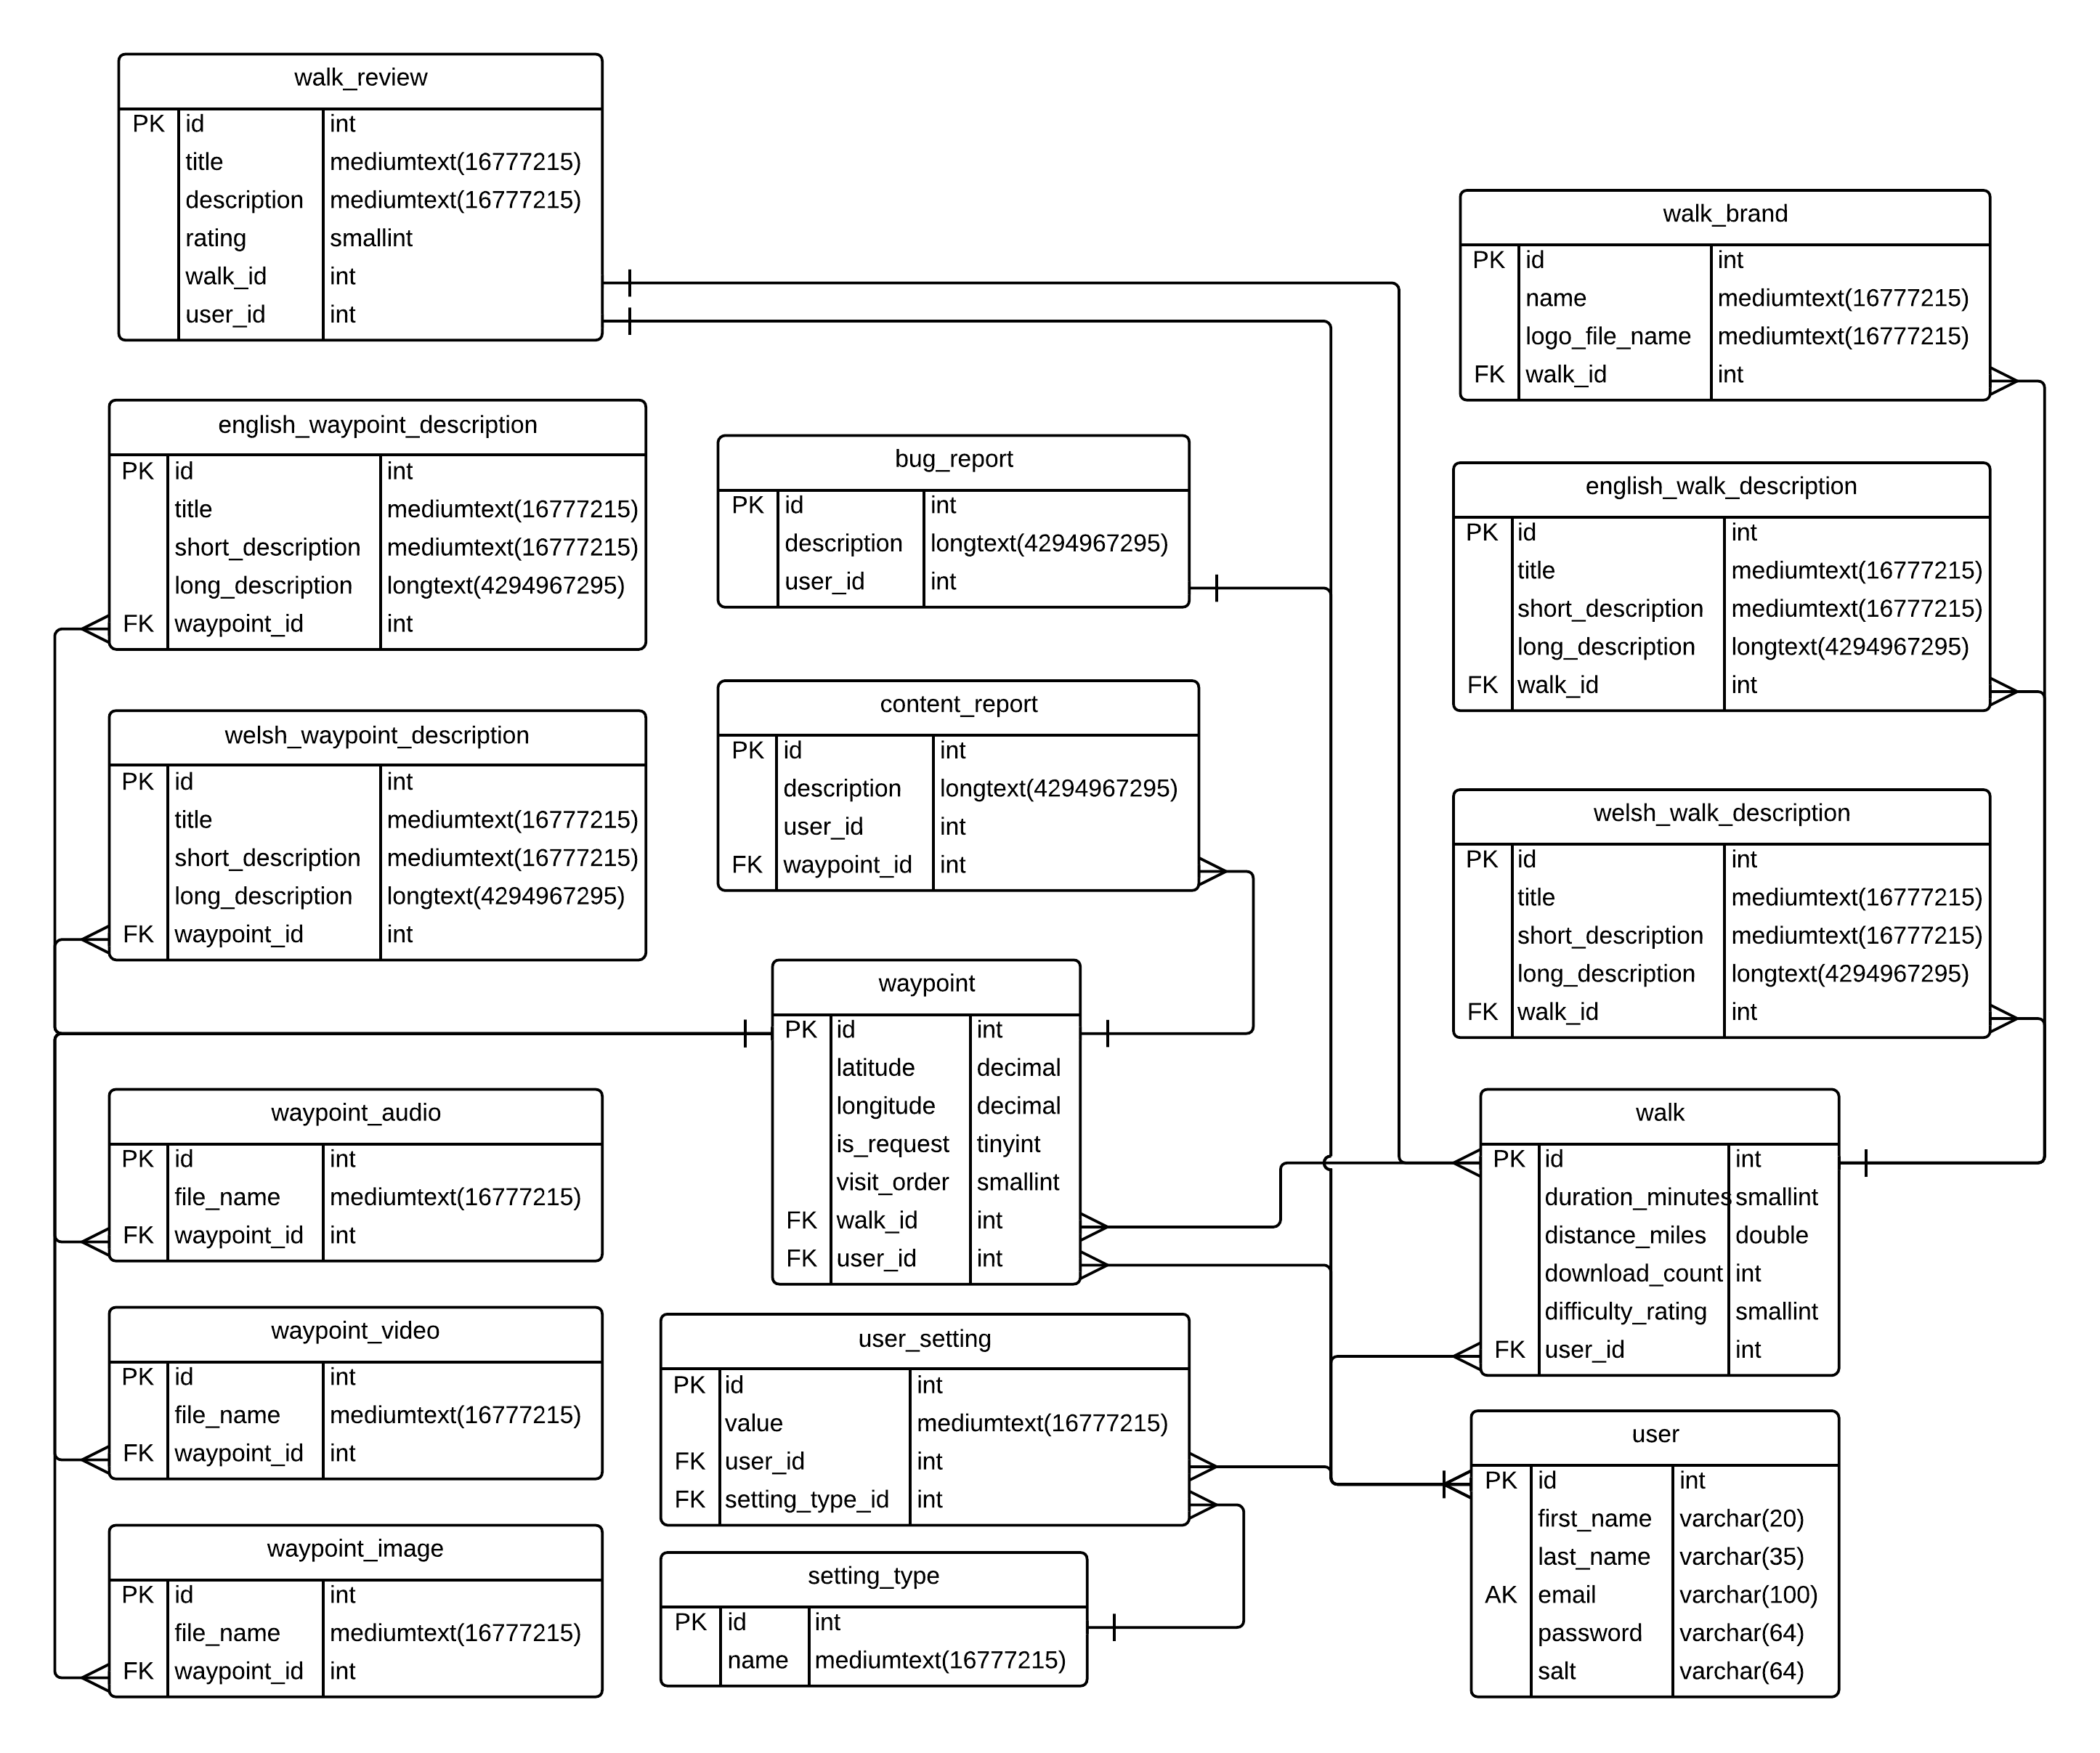
\includegraphics[angle=90, width=1\textwidth]{./img/DatabaseSchema}
\caption{Schema of the White Rock Trails relational database.}
\label{fig:DatabaseSchema}
\end{figure}

\section{API Progress}

A RESTful API has been created using the technologies discused in section \ref{sec:techAPI}. There are several important parts to the API, first it must have a coherent set of routes/urls for acces to all if its functionality, secondly it must provide a method of authenticating users and finaly it must adhear to to principles of REST as closely as possible.

\subsection{Routes}

The API is called through a series of routes, it was important to make these routes as simple and coherant as possible.

\begin{longtable}{m{0.45\textwidth}|m{0.35\textwidth}|C{0.11\textwidth}}
    \textbf{Route} & \textbf{Return value} & \textbf{Methods} \\\hline
    /walks & All walks & GET POST\\ \hline
    /walks/\$id & The walks with the ID \$id. & GET PUT DELETE\\ \hline
    /walks/\$id/waypoints & All the waypoints for the walk with the ID \$id. & GET POST\\ \hline
    /walks/\$id/waypoints/\$wid & The waypoint with the ID \$wid. & GET PUT DELETE \\ \hline
    /walks/\$id/waypoints/\$wid/images & The images for the waypoint with the ID \$wid. & GET POST \\ \hline
    /walks/\$id/waypoints/\$wid/images/\$iid & The image with the ID \$iid. & GET PUT DELETE \\ \hline
    /walks/\$id/waypoints/\$wid/audio & The audio files for the waypoint with the ID \$wid. & GET POST \\ \hline
    /walks/\$id/waypoints/\$wid/audio/\$aid & The audio file with the ID \$aid. & GET PUT DELETE \\ \hline
    /walks/\$id/waypoints/\$wid/videos & The videos for the waypoint with the ID \$wid. & GET POST \\ \hline
    /walks/\$id/waypoints/\$wid/videos/\$vid & The video with the ID \$vid. & GET PUT DELETE \\ \hline
    /users & All users. & GET POST \\\hline
    /users/\$id & The user with the ID \$id. & GET PUT DELETE \\\hline
    /users/\$id/settings & A users settings. & GET PUT \\\hline
    /session & A request to authenticate. & GET\\\hline
    /session/salt & Returns a random salt for registering a user. & GET\\\hline
    /session/salt/\$username & Get the a salt for a specific user with the username \$username. & GET\\
    \caption {The routes for the API}
    \label{routes}
\end{longtable}

The routes are structured in such a way that they help the user find the data they are looking for. They are structured similar to the database structure with waypoints belonging to walks and images, audio and videos belonging to waypoints.

To reduce load on the server any request will also return all the data that belongs to it, this means when a walk is requested it will contain all of its waypoints along with the media for each waypoint. This ensures the server is not overloaded with requests and will increase the speed of applications using the API as fewer requests are required.

Every request will respond with a JSON version of the object that the route points too. POST and PUT methods require data to be passed to the server, the API has been configured so that all request data should come in the form of a JSON object.

\lstset{language=json,
keywordstyle=\color{Maroon},
commentstyle=\color{OliveGreen},
showstringspaces=false, tabsize=4, breaklines=true, showspaces=false, stringstyle=\color{Blue}}

\begin{lstlisting}[captionpos=b, caption=JSON Return data from /walks/1, label=lst:model, frame=single]
{
	"brand":{},
	"difficulty_rating":"10",
	"distance_miles":"11.32",
	"download_count":"54",
	"duration_minutes":"35",
	"english_description":{},
	"id":"1",
	"review":[],
	"user":{},
	"user_id":"1",
	"waypoints":[],
	"welsh_description":{}
}
\end{lstlisting}

\subsubsection{CORS}
CORS, Cross-Origin Resource Sharing, limits requests to external domains unless the explicitly allow it to the same domain only. As the API is on a separate sub-domain the CORS settings of a web browser will block requests from being sent. To fix this a special OPTIONS route had to be added. It responds with a set of headers which specify which domains should be able to access the API, what methods they can use and what headers they can pass. These headers need to be passed with every request as well as the OPTIONS so they were initialised before the routes are processed meaning all requests will provide them. The API has been configured with all CORS headers and requests are allowed from any domain during the testing process.

\subsection{Authentication}

As RESTful API's are meant to be stateless, authentication must be handled in an unusual manner. The method for this was based upon the system in use at Amazon Web Services\cite{auth}. Users have a unique private key, automatically generated from their password. This private key is used to generate a signature of the data they are sending to the server. There are two compulsory headers, X-TIMESTAMP and X-USERNAME, which are used ensure there is some data to hash. The signature is sent in the header X-HASH and is then recomputed on the server using the stored private key for the user. If the two match it can be assumed that the user has the correct password and is authenticated with the appropriate permissions. This system is simpler than alternatives like OAuth which are complicated and cumbersome to implement.

The signature is generated using a keyed-hash message authentication code (HMAC) which takes the private key and the message to send (The data) and generates a hash using a specific algorithm. For the HASH we chose to use SHA1 which stands for `Secure Hashing Algorithm'. It generates a 160 bit hash which has is fairly secure but is much faster than longer alternatives such as SHA-256 or SHA-512. As the timestamp is used to validate that the request is not only correct but also recent it is highly unlikely to get two hashes which are valid at the same time even with such a small key length.

To generate the Private Key the PBKDF2 (Password-Based Key Derivation Function 2) algorithm is used. This takes in the users password and a salt which is retrieved form the database. It then preforms 1000 iterations of the SHA1 algorithm to generate a Private Key. This creates a very secure private key and makes calculating the password impossible.




\section{User Interface Design}


\subsubsection{Heuristic Evaluation}
%-- Explain how we are doing the evaluation blahblah nielsen etc.

A heuristic evaluation can be thought of as an inspection upon a product's user interface. Inspectors act as potential users, carrying out typical, everyday tasks on the product, documenting any problem they expect a user will have. Performing systematic inspections can uncover numerous issues with a product's user interface. Detecting these issues allows developers to evaluate and then make improvements to their product. A small set of evaluators carry out the inspection, judging how well the user interface meets a set of heuristic design rules. An initial set of heuristics were proposed by Nielsen and Molich in 1990~\cite{nielsen1990}. These heuristics were then refined by Nielsen and are as follows:

\begin{itemize}
  \item \textbf{Visibility of system feedback}\\ The system should always keep users informed about what is going on, through
  appropriate feedback within reasonable time.
  \item \textbf{Complexity of application}\\ The system should speak the users' language, with words, phrases and concepts
  familiar to the user, rather than system-oriented terms. Follow real-world conventions, making information appear in a natural and logical order.
  \item \textbf{Task navigation and user controls}\\ Users often choose system functions by mistake and will need a clearly marked
  ``emergency exit'' to leave the unwanted state without having to go through an extended dialogue. Support undo and redo.
  \item \textbf{Consistency and standards}\\ Users should not have to wonder whether different words, situations, or actions mean the same thing. Follow platform conventions.
  \item \textbf{Error prevention}\\ Even better than good error messages is a careful design which prevents a problem from occurring in the first place. Either eliminate error-prone conditions or check for them and present users with a confirmation option before they commit to the action.
  \item \textbf{Recognition rather than recall}\\ Minimize the user's memory load by making objects, actions, and options visible. The user should not have to remember information from one part of the dialogue to another. Instructions for use of the system should be visible or easily retrievable whenever appropriate.
  \item \textbf{Efficient to use}\\ Accelerators - unseen by the novice user -- may often speed up the interaction for the expert user such that the system can cater to both inexperienced and experienced users. Allow users to tailor frequent actions.
  \item \textbf{Simplicity and appeal}\\ Dialogues should not contain information which is irrelevant or rarely needed. Every extra unit of information in a dialogue competes with the relevant units of information and diminishes their relative visibility.
  \item \textbf{Be tolerant and reduce cost of errors}\\ Error messages should be expressed in plain language (no codes), precisely indicate the problem, and constructively suggest a solution.
  \item \textbf{Help Support}\\ Even though it is better if the system can be used without documentation, it may be necessary to provide help and documentation. Any such information should be easy to search, focused on the user's task, list concrete steps to be carried out, and not be too large.
\end{itemize}

\subsubsection{List of tasks}

Below is a list of ten tasks a typical user of the application may wish to carry out. The tasks are to be completed during the heuristic evaluation:

\begin{enumerate}
  \item Register an account
  \item Log out of an account
  \item Create a walk
  \item Search a walk
  \item Download a walk
  \item Delete a walk
  \item Add a way-point to am existing walk
  \item Edit description of an existing walk
  \item Edit way-point location of an existing walk
  \item Edit account details
\end{enumerate}

\subsubsection{Similar Products}
As part of the heuristic evaluation, two similar products were analysed and tested. The first product being TimbleOutdoors !!! and the second ViewRanger GPS CITE!!!

\subsubsection{TimbleOutdoors}

This section documents the usability problems discovered during the TimbleOutdoors evaluation.

\begin{itemize}
	\item\textbf{Usability problem: }\\
	 Visibility of system feedback heuristic violated. No indication that user has logged out.

	\item\textbf{Task attempted when problem occurred?}\\
	Task 2.

	\item\textbf{Where did the problem occur?}\\
	Settings side bar.

	\item\textbf{What suitable solution will solve the problem?}\\
	Provide a simple toast to notify a user that he/she has logged out successfully.
\end{itemize}

\line(1,0){400}

\begin{itemize}
	\item\textbf{Usability problem:}\\
	Consistency and standards. No indication of how to create a walk unless the ``Track off'' button was pressed.

	\item\textbf{Task attempted when problem occurred?}\\
	Task 3.

	\item\textbf{Where did the problem occur?}\\
	Main window.

	\item\textbf{What suitable solution will solve the problem?}\\
	Provide a standard ``Add'' icon at the top of the map view.
\end{itemize}

\line(1,0){400}

\begin{itemize}
	\item\textbf{Usability problem:}\\
	Visibility of system feedback. No indication that deletion was successful.

	\item\textbf{Task attempted when problem occurred?}\\
	Task 6.

	\item\textbf{Where did the problem occur?}\\
	My walks view.

	\item\textbf{What suitable solution will solve the problem?}\\
	Provide a simple toast to notify users that the walk has been deleted.
\end{itemize}

\line(1,0){400}

\begin{itemize}
	\item\textbf{Usability problem:}\\
	Visibility of system feedback. No indication that editing attempts were saved.

	\item\textbf{Task attempted when problem occurred?}\\
	Task 8, 9, 10.

	\item\textbf{Where did the problem occur?}\\
	Edit walk description, edit way-point location and edit account details.

	\item\textbf{What suitable solution will solve the problem?}\\
	Provide a simple toast to notify users that changes were successfully made.
\end{itemize}

\subsubsection{ViewRanger GPS}

This section documents the usability problems discovered during the ViewRanger GPS evaluation.

\begin{itemize}
	\item\textbf{Usability problem:}\\
	Error prevention. No indication whether first and last name should both be entered into first text box or separate.

	\item\textbf{Task attempted when problem occurred?}\\
	Task 1.

	\item\textbf{Where did the problem occur?}\\
	Register account window

	\item\textbf{What suitable solution will solve the problem?}\\
	Place ``First name'' and ``Last name'' above separate text boxes to avoid confusion.
\end{itemize}

\line(1,0){400}

\begin{itemize}
	\item\textbf{Usability problem:}\\
	User control and freedom. The application has no log out feature.

	\item\textbf{Task attempted when problem occurred?}\\
	Task 2.

	\item\textbf{Where did the problem occur?}\\
	Settings window.

	\item\textbf{What suitable solution will solve the problem?}\\
	Provide a button, allowing the user to log out of their account.
\end{itemize}

\line(1,0){400}

\begin{itemize}
	\item\textbf{Usability problem:}\\
	Visibility of system status. No indication that walk was successfully deleted.

	\item\textbf{Task attempted when problem occurred?}\\
	Task 6.

	\item\textbf{Where did the problem occur?}\\
	Delete walk window

	\item\textbf{What suitable solution will solve the problem?}\\
	Provide a simple toast informing the user that a walk has been deleted.
\end{itemize}

\line(1,0){400}

\begin{itemize}
	\item\textbf{Usability problem:}\\
	Match between system and the real world. ``Extend walk'' used to imply ``add a way-point''

	\item\textbf{Task attempted when problem occurred?}\\
	Task 7.

	\item\textbf{Where did the problem occur?}\\
	Main window.

	\item\textbf{What suitable solution will solve the problem?}\\
	Correct the terminology used in order to prevent confusion.
\end{itemize}

\line(1,0){400}

\begin{itemize}
	\item\textbf{Usability problem:}\\
	Visibility of system status. No indication that alterations were successful.

	\item\textbf{Task attempted when problem occurred?}\\
	Task 8 and 9.

	\item\textbf{Where did the problem occur?}\\
	Edit walk description window and edit way-point location window.

	\item\textbf{What suitable solution will solve the problem?}\\
	Provide simple toast to inform the user his/her update was successful.
\end{itemize}

\line(1,0){400}

\begin{itemize}
	\item\textbf{Usability problem:}\\
	User control and freedom. No ability to edit account details, but user may sign in or register (whilst already signed in).

	\item\textbf{Task attempted when problem occurred?}\\
	Task 10.

	\item\textbf{Where did the problem occur?}\\
	Account activation window.

	\item\textbf{What suitable solution will solve the problem?}\\
	Provide a feature allowing users to edit their account.
\end{itemize}


\subsubsection{Prototype Designs}

Prototyping is an important aspect of software development. Creating prototype designs allows developers to produce a simplified version of a potential product. This means feedback can be gathered from users early in the project. It also allows developers to assess their prototype product, ensuring it meets the requirements set out by a client. This section of the document will analyse two prototype stages. First, a low level design that includes basic application layout and simple features. The second prototype design shows the application during the development stage and includes additional features. A heuristic evaluation of the second prototype will also be provided.

\subsubsection{Prototype 1}

The first prototype began as a series hand drawn template designs. These basic mock-ups were adapted to create a more impressive prototype design using Evolus Pencil, an open source user interface design tool that allows for professional prototype designs to be produced~\cite{pencil}.

\begin{figure}[H]
\begin{center}
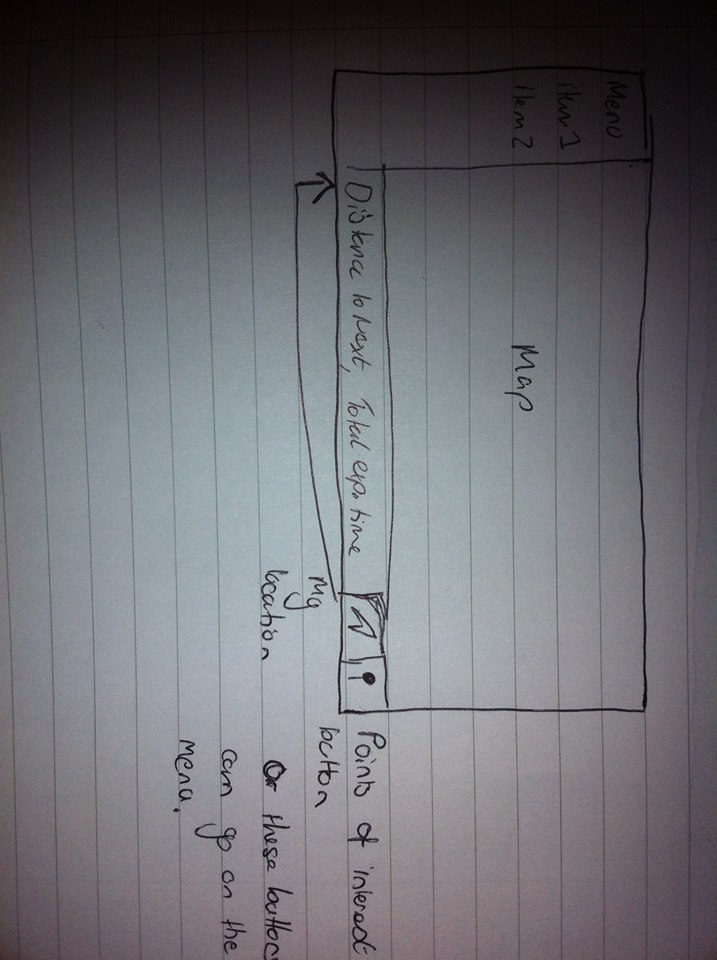
\includegraphics[angle = 90, width=.8\linewidth]{./img/hand_drawn.jpg}
\caption{Walk View - Hand drawn Design}
\label{fig:handDrawn}
\end{center}
\end{figure}

Figure~\ref{fig:handDrawn} illustrates an original mock-up design for a typical walk interface. The majority of the interface is made up of a map, displaying the user's current location. A side view will include a menu option and a list of way-points relevant to a specific walk trail. A footer bar will include information about distance and time expected to next point of interest. This simple design was used to create the second stage of prototype 1.

\begin{figure}[H]
\begin{center}
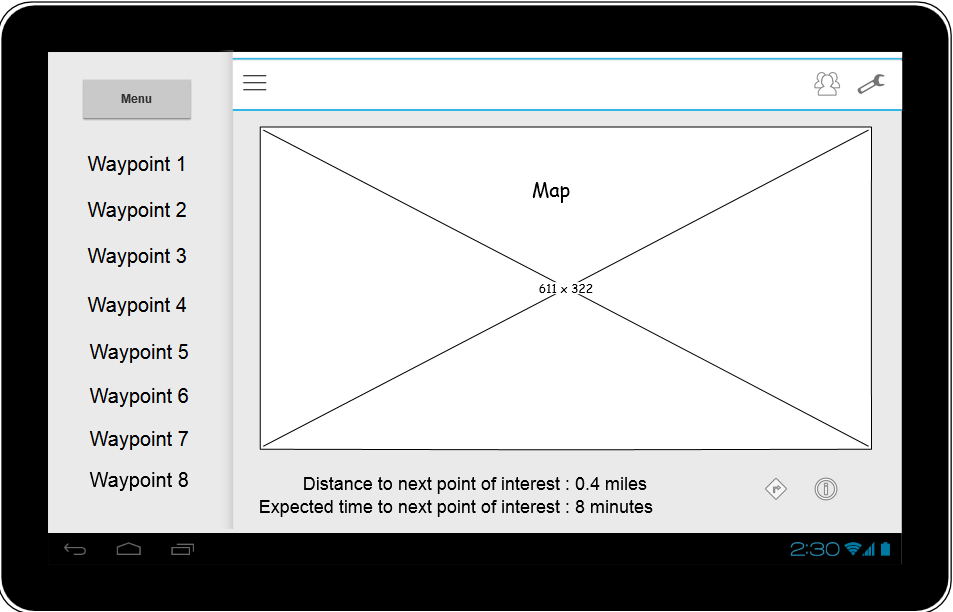
\includegraphics[width=12cm]{./img/pencil_proto1.jpg}
\caption{Walk View - Evolus Pencil Design}
\label{fig:walkView}
\end{center}
\end{figure}

\begin{figure}[H]
\begin{center}
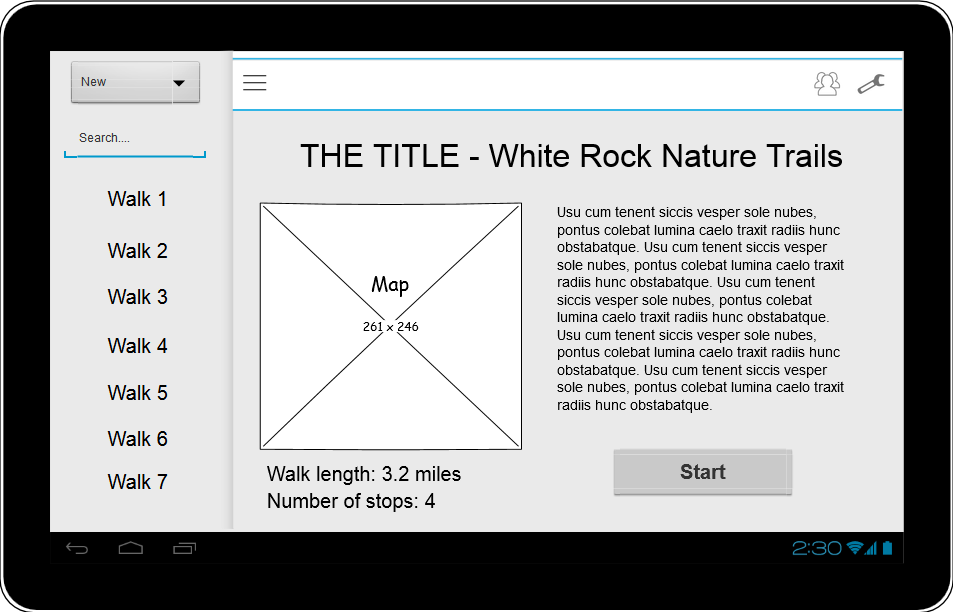
\includegraphics[width=12cm]{./img/pencil_choose_walk.jpg}
\caption{Choose A Walk View - Evolus Pencil Design}
\label{fig:chooseWalk}
\end{center}
\end{figure}

Similar to ``Walk View``, the ``Choose A Walk View''(Figure~\ref{chooseWalk}) includes of a side bar, header bar. This interface view allows the user to scroll through a list of walks and be presented with information about each walk, such as walk name, description, map location, length of walk and the number of walk points of interests (way-points). This interface view also includes a button, allowing the user to begin a chosen walk. For additional prototype 1 designs, see Appendix x.

\subsubsection{Prototype 2}

\begin{figure}[h!]
\begin{center}
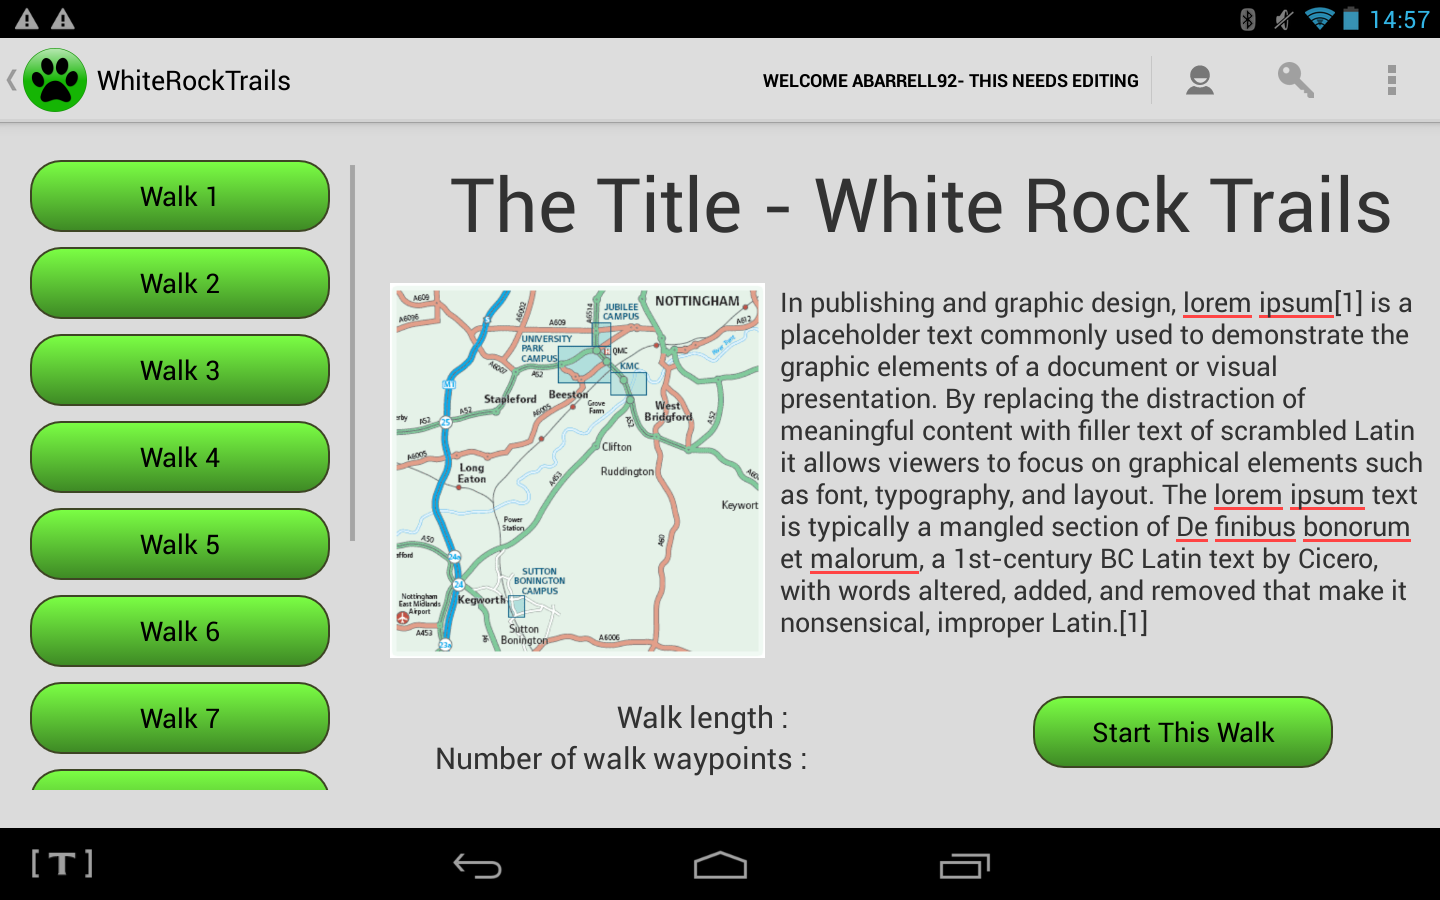
\includegraphics[width=12cm]{./img/app_choose_walk.png}
\caption{Choose A Walk View - Android Application Design}
\end{center}
\end{figure}


\begin{figure}[h!]
\begin{center}
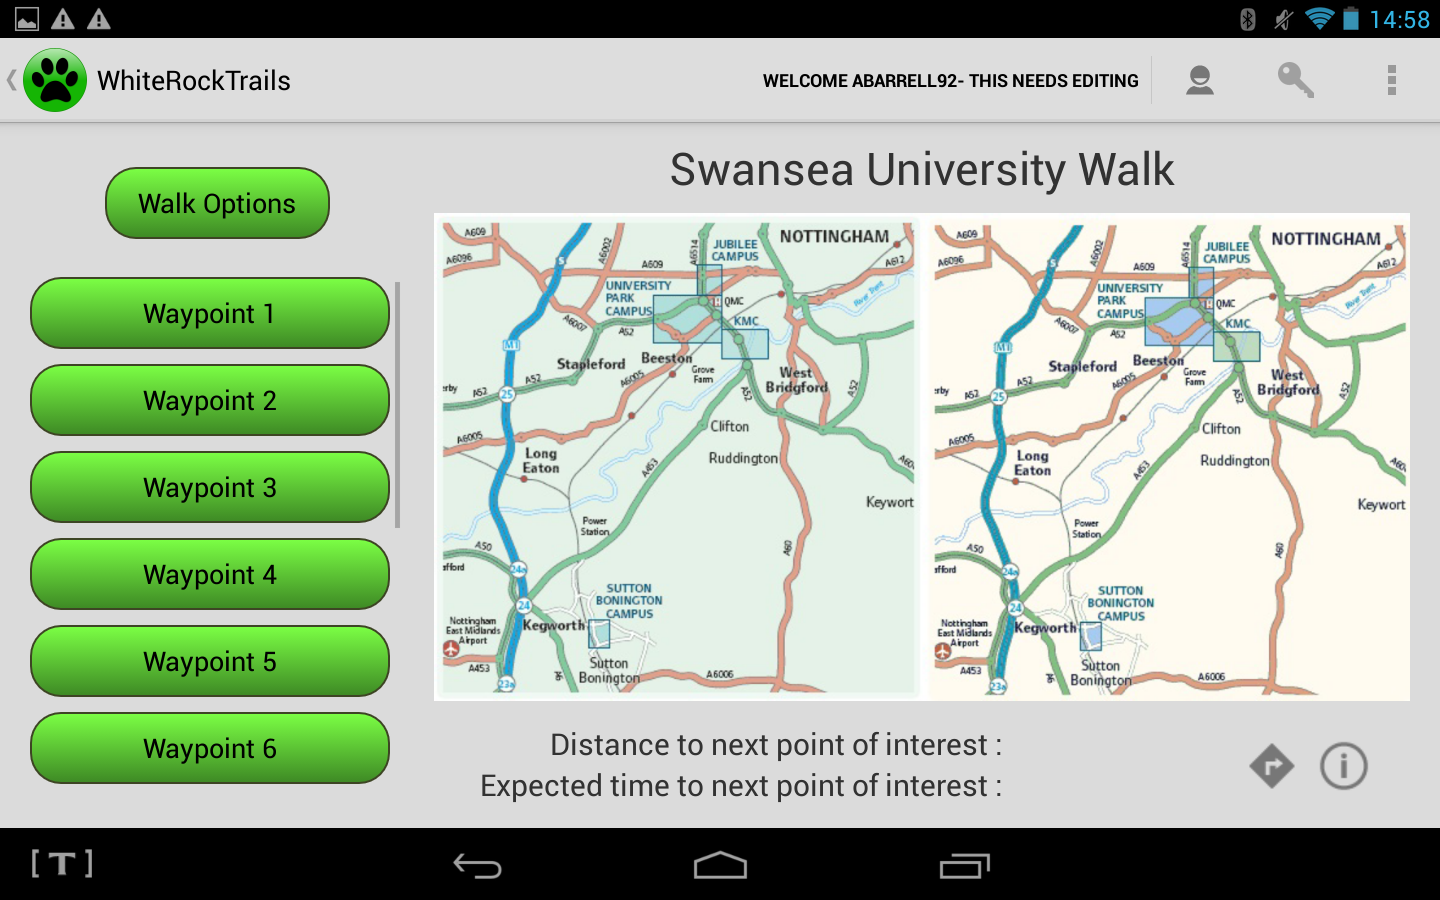
\includegraphics[width=12cm]{./img/app_walk_view.png}
\caption{Walk View - Android Application Design}
\end{center}
\end{figure}

Prototype 2 was created using Eclipse ADT CITE!!!!!!!!. Through the use of XML CITE!!!, a series of application interface designs were produced. Figure x and y are both improvements of interfaces described in section X, prototype 1. When minor functionality was added to prototype 2, a heuristic evaluation was carried out. The following section documents the usability problems discovered during the White Rock evaluation.

\begin{itemize}
	\item\textbf{Usability problem:}\\
	Visibility of system status. Log out doesn't have a confirmation feature.

	\item\textbf{Task attempted when problem occurred?}\\
	Task 2.

	\item\textbf{Where did the problem occur?}\\
	At the application action bar when signed in.

	\item\textbf{What suitable solution will solve the problem?}\\
	Simply apply a confirmation dialogue fragment when the "log out" icon is pressed.

\end{itemize}

\line(1,0){400}

\begin{itemize}
	\item\textbf{Usability problem:}\\
	Visibility of system status. No confirmation that a walk was successfully created.

	\item\textbf{Task attempted when problem occurred?}\\
	Task 3.

	\item\textbf{Where did the problem occur?}\\
	Create walk window.

	\item\textbf{What suitable solution will solve the problem?}\\
	Add a toast to notify the user that a walk was successfully created.

\end{itemize}

\line(1,0){400}

\begin{itemize}
	\item\textbf{Usability problem:}\\
	Visibility of system status. No confirmation edit was successful.

	\item\textbf{Task attempted when problem occurred?}\\
	Task 8, 9 and 10.

	\item\textbf{Where did the problem occur?}\\
	Edit description of existing walk, edit way-point description of existing walk and edit account details.

	\item\textbf{What suitable solution will solve the problem?}\\
	Add a toast to notify user that their changes were accepted and successful.

\end{itemize}

From the above evaluation, it is evident that the application is still at the latter prototype stages. Minor functionality, such as toast notifications and dialogue fragments, are to be added at a later date, ensuring the application conforms to Neilsen's heuristics.



\section{Android Application Progress}
\lstset{language=Java,
keywordstyle=\color{Maroon},
commentstyle=\color{OliveGreen},
showstringspaces=false, tabsize=4, breaklines=true, showspaces=false, stringstyle=\color{Blue}}
The development of the Android application is progressing well and has been minimally affected by risks, both expected and unexpected. To achieve the goals of the project, the application has to be capable of saving and loading data to and from a local database, which will then synchronise with the remote database - this is achieved via a ContentProvider, seen in Section~\ref{sec:contentprovier}; the client also requested Google Maps be implemented, the progress of which can be seen in Section~\ref{sec:googlemaps}; as the application allows users to log-in and personalise their experience an authentication system has been created, seen in Section~\ref{sec:authorisation}. Tying all of these features together is the SyncAdapter, seen in Section~\ref{sec:syncAdapter}, which will allow for efficient synchronisation of data to and from the server. Finally, fragments and activities have been created to control the flow of the program, along with relevant layouts and graphics, which can be seen in Section~\ref{sec:fragments}. All of these systems, when completed, will meet the requirements shown in Section 4.1.2 of the Milestone 1 document~\cite{initialDoc}. It should be noted that all code samples seen in the following sections have been modified for this document and do not represent the quality of production code nor adhere to all of the guidelines stated in Section~\ref{sec:codingguidelines}.

\subsection{ContentProvider}
\label{sec:contentprovier}
The ContentProvider provides valuable functionality when synchronising with the server and allowing for other applications to, potentially, access the application's database. It consists of four components. Firstly, there is the DbSchema class, this interface class contains all of the SQL used to create the table and constants such as table names. Next comes the DatabaseHandler class, an extension of the Android SQLiteOpenHelper class, which creates the database and contains the strategy for deleting and upgrading the database; it is also responsible for opening and closing connections to the database. The WhiteRockContract class provides an API for foreign applications to access available data, without this the ContentProvider does not achieve anything. Finally, there is the WhiteRockContentProvider class itself, this class is responsible for inserting, deleting, updating and querying the database.

\subsubsection{Database Schema}
The DbSchema class is an interface which is strictly used for referencing constants, such as table names, and strings containing the SQL used to create each table in the database. Example code can be seen in Listing~\ref{lst:dbSchema}.

\begin{lstlisting}[captionpos=b, caption=DbSchema Snippet, label=lst:dbSchema, frame=single]
// Example code snippet from DbSchema.java

String VIEW_WAYPOINT_WITH_ENGLISH_DESCR = "waypoint_and_english";

String CREATE_TABLE_WALK =
		"CREATE TABLE `walk` ("
		+"_id INTEGER PRIMARY KEY AUTOINCREMENT ,"
		+"duration_minutes INT,"
		+"distance_miles REAL,"
		+"download_count INT,"
        +"difficulty_rating INT,"
		+"user_id INT"
		+")";

String CREATE_TABLE_WALK_BRAND =
		"CREATE TABLE `walk_brand` ("
		+"_id INTEGER PRIMARY KEY AUTOINCREMENT ,"
		+"name TEXT,"
		+"logo_file_name TEXT,"
        +"walk_id INT"
		+")";

\end{lstlisting}

\subsubsection{DatabaseHandler}
Responsible for creating, deleting and upgrading the database, as well as opening and closing connections, the DatabaseHandler class is vital for both maintaining the database and interfacing with it.

Listing~\ref{lst:dbHandler} provides a snippet of the code used during the creation of a DatabaseHandler instance and how it uses the DbSchema to create the database.

\begin{lstlisting}[captionpos=b, caption=DatabaseHandler Snippet, label=lst:dbHandler, frame=single]
public DatabaseHandler(Context context) {
	super(context, DB_NAME, null, DB_VERSION);

    // Find the correct path based on Android version.
    if (android.os.Build.VERSION.SDK_INT >= Build.VERSION_CODES.JELLY_BEAN_MR1) {
        DB_PATH = context.getApplicationInfo().dataDir + "/databases/";
    } else {
        DB_PATH = "/data/data/" + context.getPackageName() + "/databases/";
    }
    Log.d(TAG,"DB Path is: " + DB_PATH+DB_NAME);
    Log.d(TAG, "Version Number: " + android.os.Build.VERSION.SDK_INT);
    this.mContext = context;
}

@Override
public void onCreate(SQLiteDatabase db) {
    Log.d(TAG, "CREATING");
    // create User tables
    db.execSQL(DbSchema.CREATE_TABLE_USER);
    db.execSQL(DbSchema.CREATE_TABLE_SETTING_TYPE);
    db.execSQL(DbSchema.CREATE_TABLE_USER_SETTINGS);

    // Create Walk Tables
    db.execSQL(DbSchema.CREATE_TABLE_WALK);
    db.execSQL(DbSchema.CREATE_TABLE_WALK_BRAND);
    db.execSQL(DbSchema.CREATE_TABLE_WALK_REVIEW);
    db.execSQL(DbSchema.CREATE_TABLE_ENGLISH_WALK_DESCR);
    db.execSQL(DbSchema.CREATE_TABLE_WELSH_WALK_DESCR);
}
\end{lstlisting}

\subsubsection{WhiteRockContract}
The WhiteRockContract class is the API which all applications, including this one, must use to access the ContentProvider. The class itself is relatively simple, providing constant values for the Authority and Content URI's required to access the data. The ContentProvider accesses data from the database by being passed a URI in the format content://authority//path\_to\_type. In this implementation the authority is ``uk.ac.swan.digitaltrails'' the path\_to\_type variable points to a table name, such as ``walk''. An example of this, for the ``bug\_report'' table, can be seen in Listing~\ref{lst:contract}.

\begin{lstlisting}[captionpos=b, caption=WhiteRockContract Snippet, label=lst:contract, frame=single]
public class WhiteRockContract {

	public static final String AUTHORITY = "uk.ac.swan.digitaltrails";
	public static final Uri CONTENT_URI = Uri.parse("content://" + AUTHORITY);


	/**
	 * Constants for Bug Report table.
	 * @author Lewis Hancock
	 *
	 */
	public static final class BugReport implements ReportColumns {
		public static final Uri CONTENT_URI = Uri.withAppendedPath(
				WhiteRockContract.CONTENT_URI, "bug_report");

		public static final String CONTENT_TYPE = ContentResolver.CURSOR_DIR_BASE_TYPE +
				"vnd.uk.ac.swan.digitaltrails.bug_report";

		public static final String CONTENT_TYPE_DIR = ContentResolver.CURSOR_ITEM_BASE_TYPE +
				"vnd.uk.ac.swan.digitaltrails.bug_report";

		public static final String SORT_ORDER_DEFAULT = ID + " ASC";

		public static final String[] PROJECTION_ALL = {ID, DESCRIPTION, USER_ID};

	}
	// rest of code omitted
}
\end{lstlisting}

\subsubsection{WhiteRockContentProvider}
The WhiteRockContentProvider class is where all of the components come together. A URIMatcher is created to ensure that the correct data is accessed, according to the content URI passed. Based on the call to the ContentProvider (insert, update, delete, query), the URI passed is matched via the URIMatcher and the operation carried out on the correct data in the correct table. Examples of each operation can be seen in Listing~\ref{lst:contentprovider}.

\begin{lstlisting}[captionpos=b, caption=WhiteRockContentProvider Snippet, label=lst:contentprovider, frame=single]
private static UriMatcher buildUriMatcher() {
    final UriMatcher matcher = new UriMatcher(UriMatcher.NO_MATCH);
    final String authority = WhiteRockContract.AUTHORITY;
    matcher.addURI(authority, "walk", WALK_LIST);
    matcher.addURI(authority, "walk/#", WALK_ID);
    matcher.addURI(authority, "english_walk_description", ENGLISH_WALK_DESCR_LIST);
    matcher.addURI(authority, "english_walk_description/#", ENGLISH_WALK_DESCR_ID);
    matcher.addURI(authority, "welsh_walk_description", WELSH_WALK_DESCR_LIST);
    matcher.addURI(authority, "welsh_walk_description/#", WELSH_WALK_DESCR_ID);
}

@Override
public boolean onCreate() {
    Context context = getContext();
    mDbHandler = new DatabaseHandler(context);
    return true;
}

@Override
public int delete(Uri uri, String selection, String[] selectionArgs) {
    SQLiteDatabase db = mDbHandler.getWritableDatabase();
    int deleteCount = 0;
    String idStr;
    String where;

    switch (URI_MATCHER.match(uri)) {
    case WALK_LIST:
        deleteCount = db.delete(DbSchema.TABLE_WALK, selection, selectionArgs);
        break;
    case WALK_ID:
        idStr = uri.getLastPathSegment();
        where = WhiteRockContract.Walk._ID + " = " + idStr;
        if (!TextUtils.isEmpty(selection)) {
            where += " AND " + selection;
        }
        deleteCount = db.delete(DbSchema.TABLE_WALK, where, selectionArgs);
        break;
        // Rest of code omitted.
    }
    return deleteCount;
}

@Override
public Uri insert(Uri uri, ContentValues values) {
    SQLiteDatabase db = mDbHandler.getWritableDatabase();
    long id = 0;
    switch (URI_MATCHER.match(uri)) {
    case WALK_LIST:
        id = db.insert(DbSchema.TABLE_WALK,
                      null,
                      values);
        db.close();
        return getUriForId(id, uri);
    case WAYPOINT_LIST:
        id = db.insert(DbSchema.TABLE_WAYPOINT,
                      null,
                      values);
        db.close();
        Log.d(TAG, "Attempting insert into waypoint table");
        return getUriForId(id, uri);

        // Rest of code omitted
    }
}

@Override
public Cursor query(Uri uri, String[] projection, String selection, String[] selectionArgs,
        String sortOrder) {
    SQLiteDatabase db = mDbHandler.getReadableDatabase();
    SQLiteQueryBuilder builder = new SQLiteQueryBuilder();
    String queryString;
    boolean useAuthorityUri = false;
    switch (URI_MATCHER.match(uri)) {
    case WALK_LIST:
        builder.setTables(DbSchema.TABLE_WALK);
        if (TextUtils.isEmpty(sortOrder)) {
            sortOrder = WhiteRockContract.Walk.SORT_ORDER_DEFAULT;
        }
        break;
    case WALK_ID:
        builder.setTables(DbSchema.TABLE_WALK);
        builder.appendWhere(WhiteRockContract.Walk._ID + " = " + uri.getLastPathSegment());
        break;
        // rest of code omitted
    }
    Log.d(TAG, builder.getTables());
    Cursor cursor = builder.query(db, projection, selection, selectionArgs, null, null, sortOrder);
    if (useAuthorityUri) {
        cursor.setNotificationUri(getContext().getContentResolver(), WhiteRockContract.CONTENT_URI);
    } else {
        cursor.setNotificationUri(getContext().getContentResolver(), uri);
    }
    return cursor;
}

@Override
public int update(Uri uri, ContentValues values, String selection, String[] selectionArgs) {

    SQLiteDatabase db = mDbHandler.getWritableDatabase();
    int updateCount = 0;
    String idStr;
    String where;

    switch(URI_MATCHER.match(uri)) {
    case WALK_LIST:
        updateCount = db.update(DbSchema.TABLE_WALK, values, selection, selectionArgs);
        break;
    case WALK_ID:
        idStr = uri.getLastPathSegment();
        where = WhiteRockContract.Walk._ID + " = " + idStr;
        if (!TextUtils.isEmpty(selection)) {
            where += " AND " + selection;
        }
        updateCount = db.update(DbSchema.TABLE_WALK, values, where, selectionArgs);
        break;
        // rest of code omitted.
    }
    return updateCount;
}

\end{lstlisting}

\subsubsection{Using the ContentProvider}
The ContentProvider is currently being used, in conjunction with a CursorLoader, to query the database for walk names to choose a walk and, when a walk has been chosen, the waypoint details of that walk. The CursorLoader is an asynchronous loader, allowing data to be loaded in a different thread than the User Interface thread. This is great for loading the user interface whilst the data is loading. Relevant code for loading data, in this example the titles of each walk and their details, can be seen in Listing~\ref{lst:walkListFragment}.

\begin{lstlisting}[captionpos=b, caption=WalkListFragment Snippet, label=lst:walkListFragment, frame=single]

public class WalkListFragment extends ListFragment
	implements LoaderCallbacks<Cursor>, OnQueryTextListener {

	// Non-relevant code omitted.

	static String [] WALK_SUMMARY_PROJECTION = {WhiteRockContract.EnglishWalkDescriptions._ID, WhiteRockContract.EnglishWalkDescriptions.TITLE, WhiteRockContract.EnglishWalkDescriptions.WALK_ID };

	@Override
	public void onActivityCreated(Bundle savedInstanceState) {
		super.onActivityCreated(savedInstanceState);

		//setHasOptionsMenu(true);
		setEmptyText("No Walks");	//TODO load this from resource.
		mAdapter = new SimpleCursorAdapter(getActivity(), mLayout, null,
					new String[] {WhiteRockContract.EnglishWalkDescriptions.TITLE },
					new int[] {android.R.id.text1}, 0);
		setListAdapter(mAdapter);
		setListShown(false);
		// Load the data!
		getLoaderManager().initLoader(0, null, this);
	}


	@Override
	public Loader<Cursor> onCreateLoader(int id, Bundle args) {
		Uri baseUri;
		if (mCurFilter != null) {
			baseUri = Uri.withAppendedPath(WhiteRockContract.CONTENT_URI, Uri.encode(mCurFilter));
		} else {
			baseUri = WhiteRockContract.EnglishWalkDescriptions.CONTENT_URI;
		}

		String select = "((_id))";
		return new CursorLoader(getActivity(), baseUri, WALK_SUMMARY_PROJECTION, select, null, WhiteRockContract.EnglishWalkDescriptions.WALK_ID + " COLLATE LOCALIZED ASC");
	}

	@Override
	public void onLoadFinished(Loader<Cursor> loader, Cursor data) {
		mAdapter.swapCursor(data);

		if (isResumed()) {
			setListShown(true);
		} else {
			setListShownNoAnimation(true);
		}

	}

	@Override
	public void onLoaderReset(Loader<Cursor> arg0) {
		mAdapter.swapCursor(null);
	}
}
\end{lstlisting}

All of the code (and more) in the above sections results in the screens and interactions seen in Figures~\ref{fig:walkListFragment} and~\ref{fig:googleContentLoader} being available in the application at the time of writing. This code is now completed, unless it becomes clear that we need access to other areas of the database.

\begin{figure}[H]
\centering
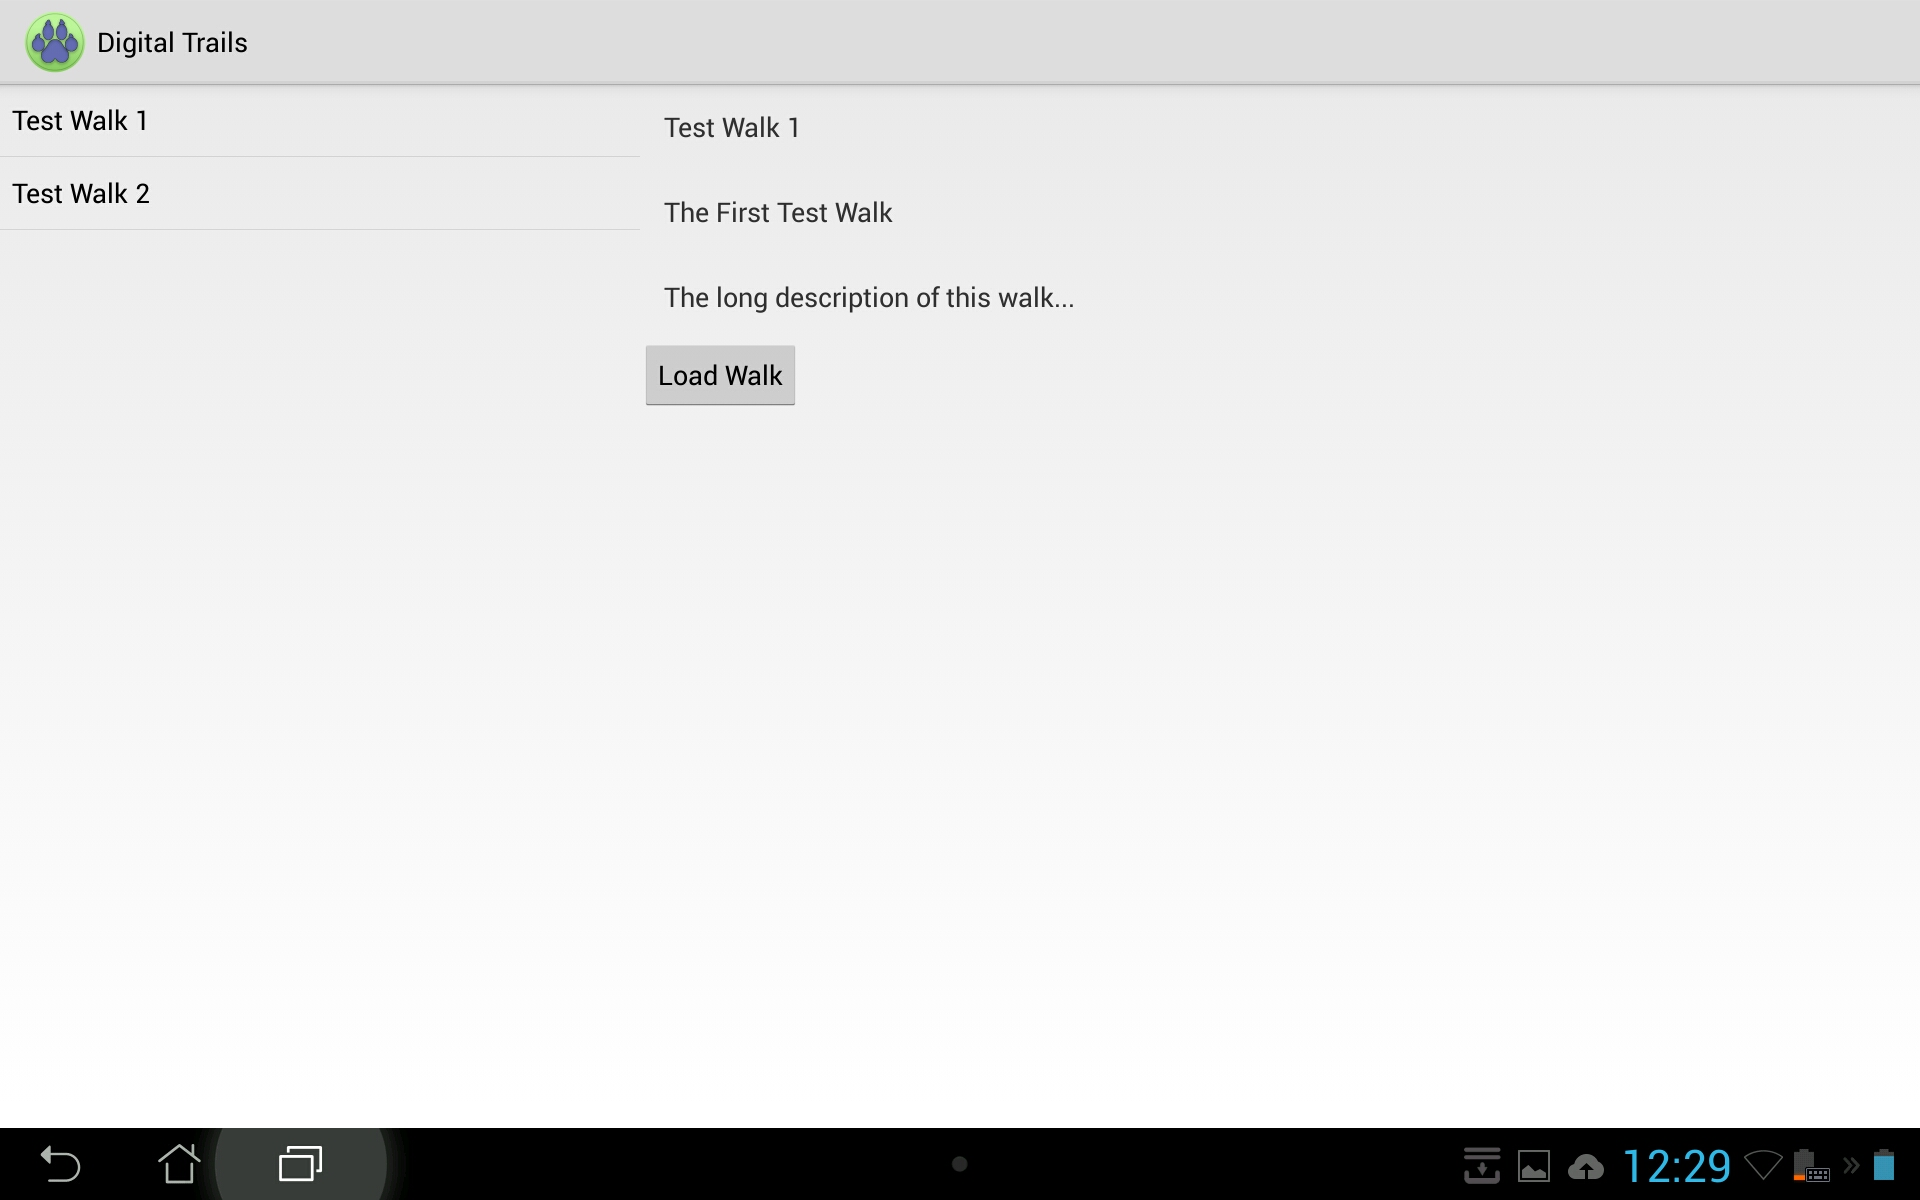
\includegraphics[width=.7\linewidth]{walkListFragment.jpg}
\caption{Screenshot of WalkListFragment Fragment loading walk details from the database.}
\label{fig:walkListFragment}
\end{figure}


\begin{figure}[H]
\centering
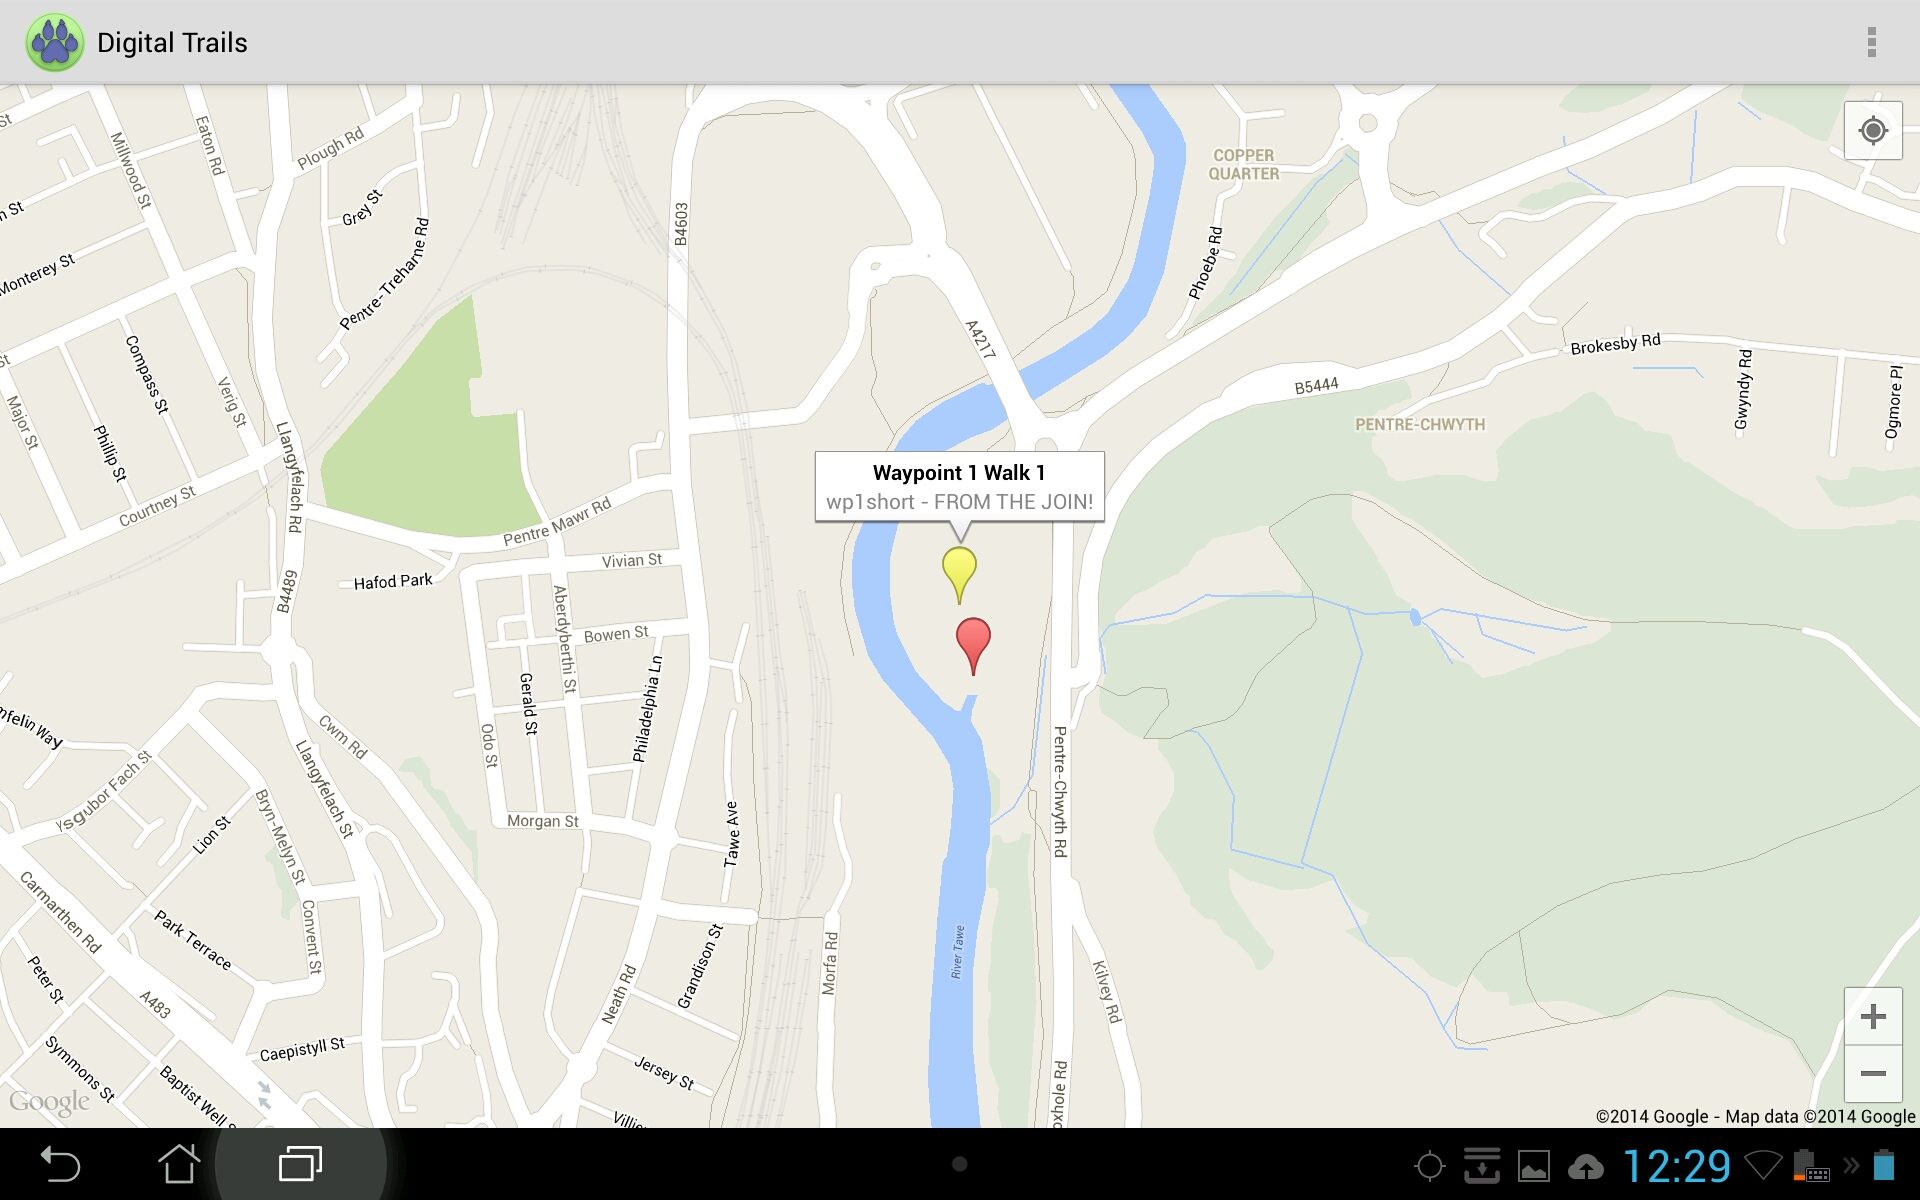
\includegraphics[width=.7\linewidth]{googleMapsContentLoader.jpg}
\caption{Screenshot of the MapActivity displaying waypoint details from the database.}
\label{fig:googleContentLoader}
\end{figure}


\subsection{Google Maps}
\label{sec:googlemaps}
Currently the Google Maps API has been integrated at a basic level. The user can select a walk and the correct data will be displayed on the Map, with tappable waypoint markers. After tapping a marker a small information area (InfoWindow) will appear, this gives the waypoint title and the short description of it. Tapping on this area will display a large dialog, displaying all the information available for that waypoint. These interactions can be seen in Figures~\ref{fig:googleContentLoader} and~\ref{fig:wpInfoDialog}.

\begin{figure}[H]
\centering
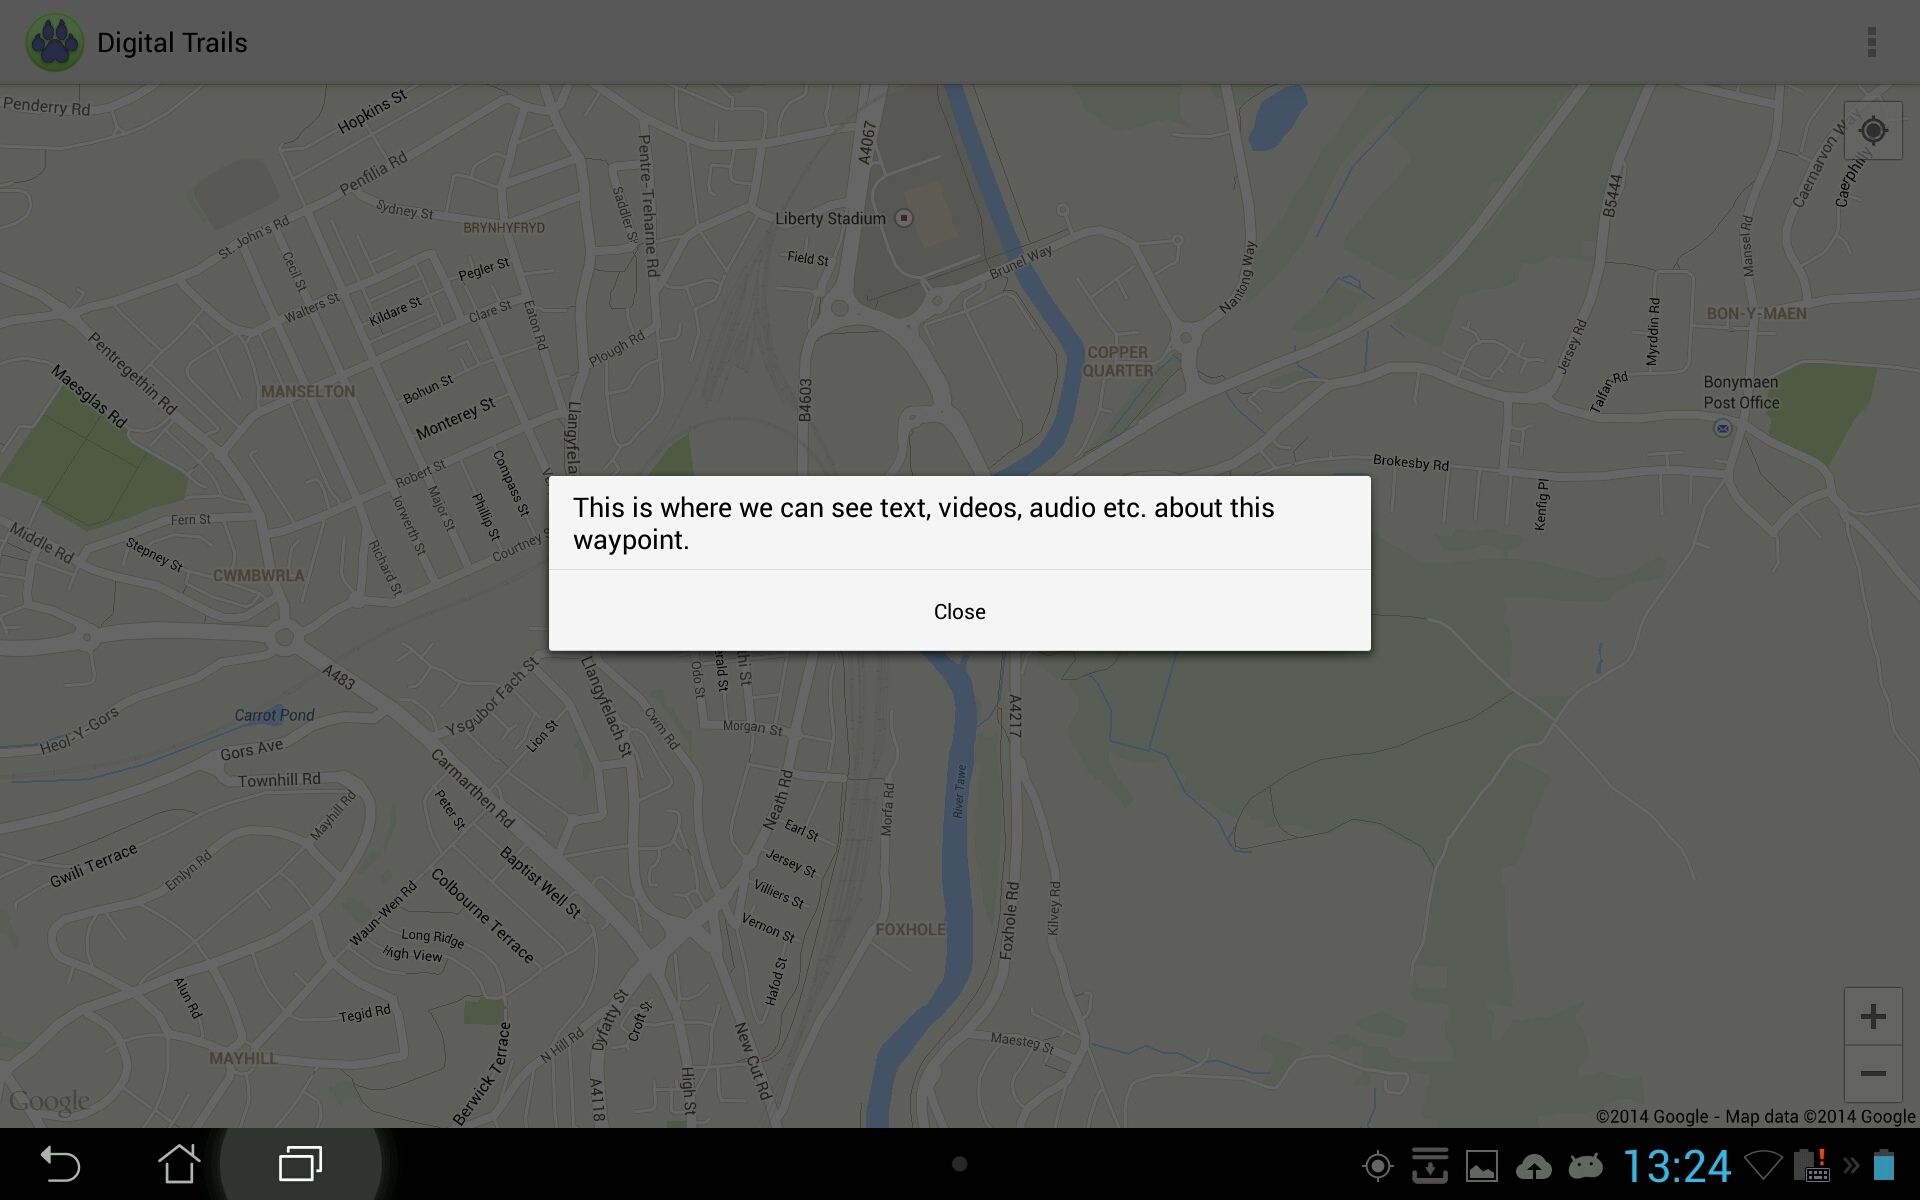
\includegraphics[width=.7\linewidth]{wpInfoDialog.jpg}
\caption{Screenshot of the MapActivity Information Dialog.}
\label{fig:wpInfoDialog}
\end{figure}

Users may also change the style of the map to ``Normal'', ``Hybrid'' or ``Satellite''; rotate, zoom, pan and tilt the map with gestures and zoom the map in and out and find the user's current location with on-screen buttons. These can be see in Figures~\ref{fig:mapOptions} and~\ref{fig:userLocation}.

\begin{figure}[H]
\centering
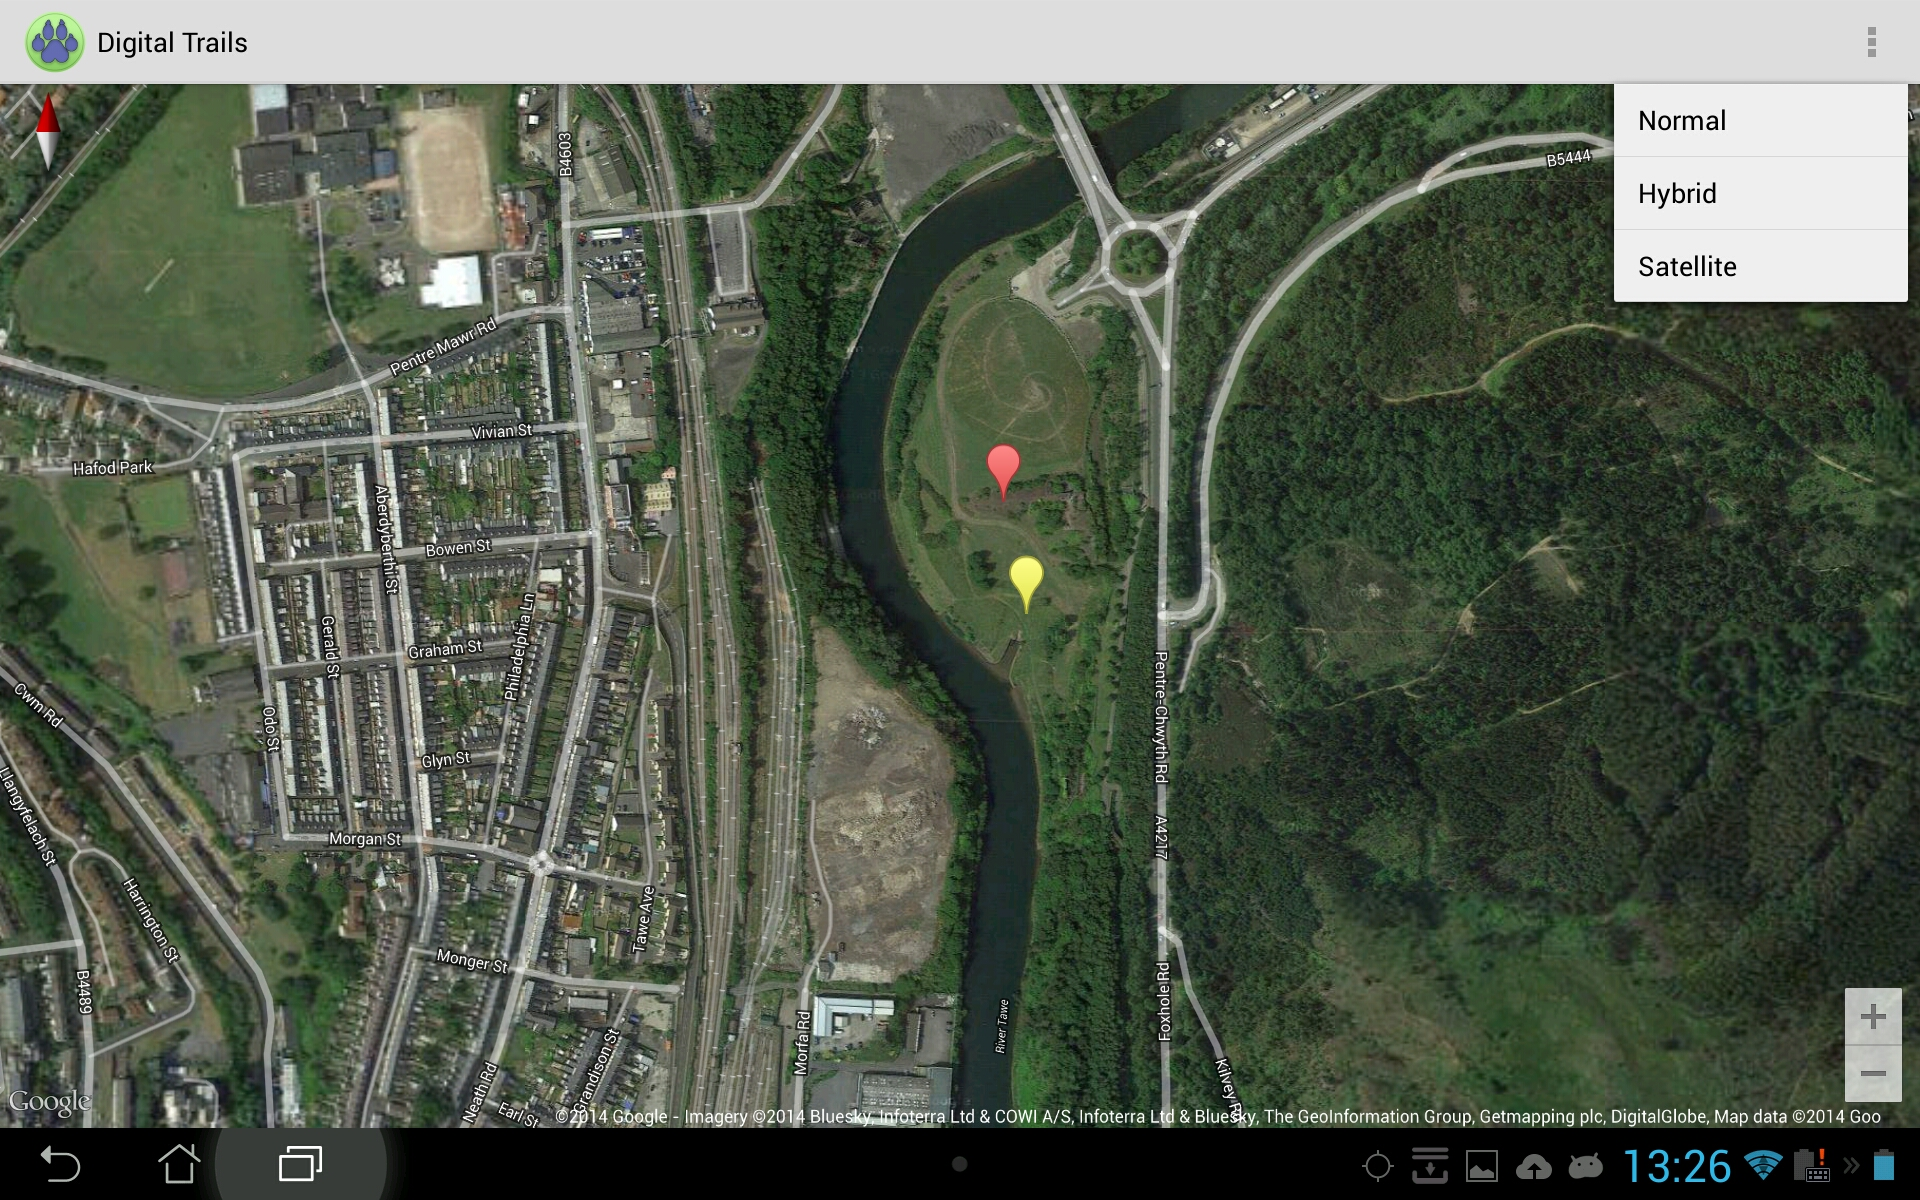
\includegraphics[width=.7\linewidth]{mapOptions.jpg}
\caption{Screenshot of the MapActivity map options.}
\label{fig:mapOptions}
\end{figure}

\begin{figure}[H]
\centering
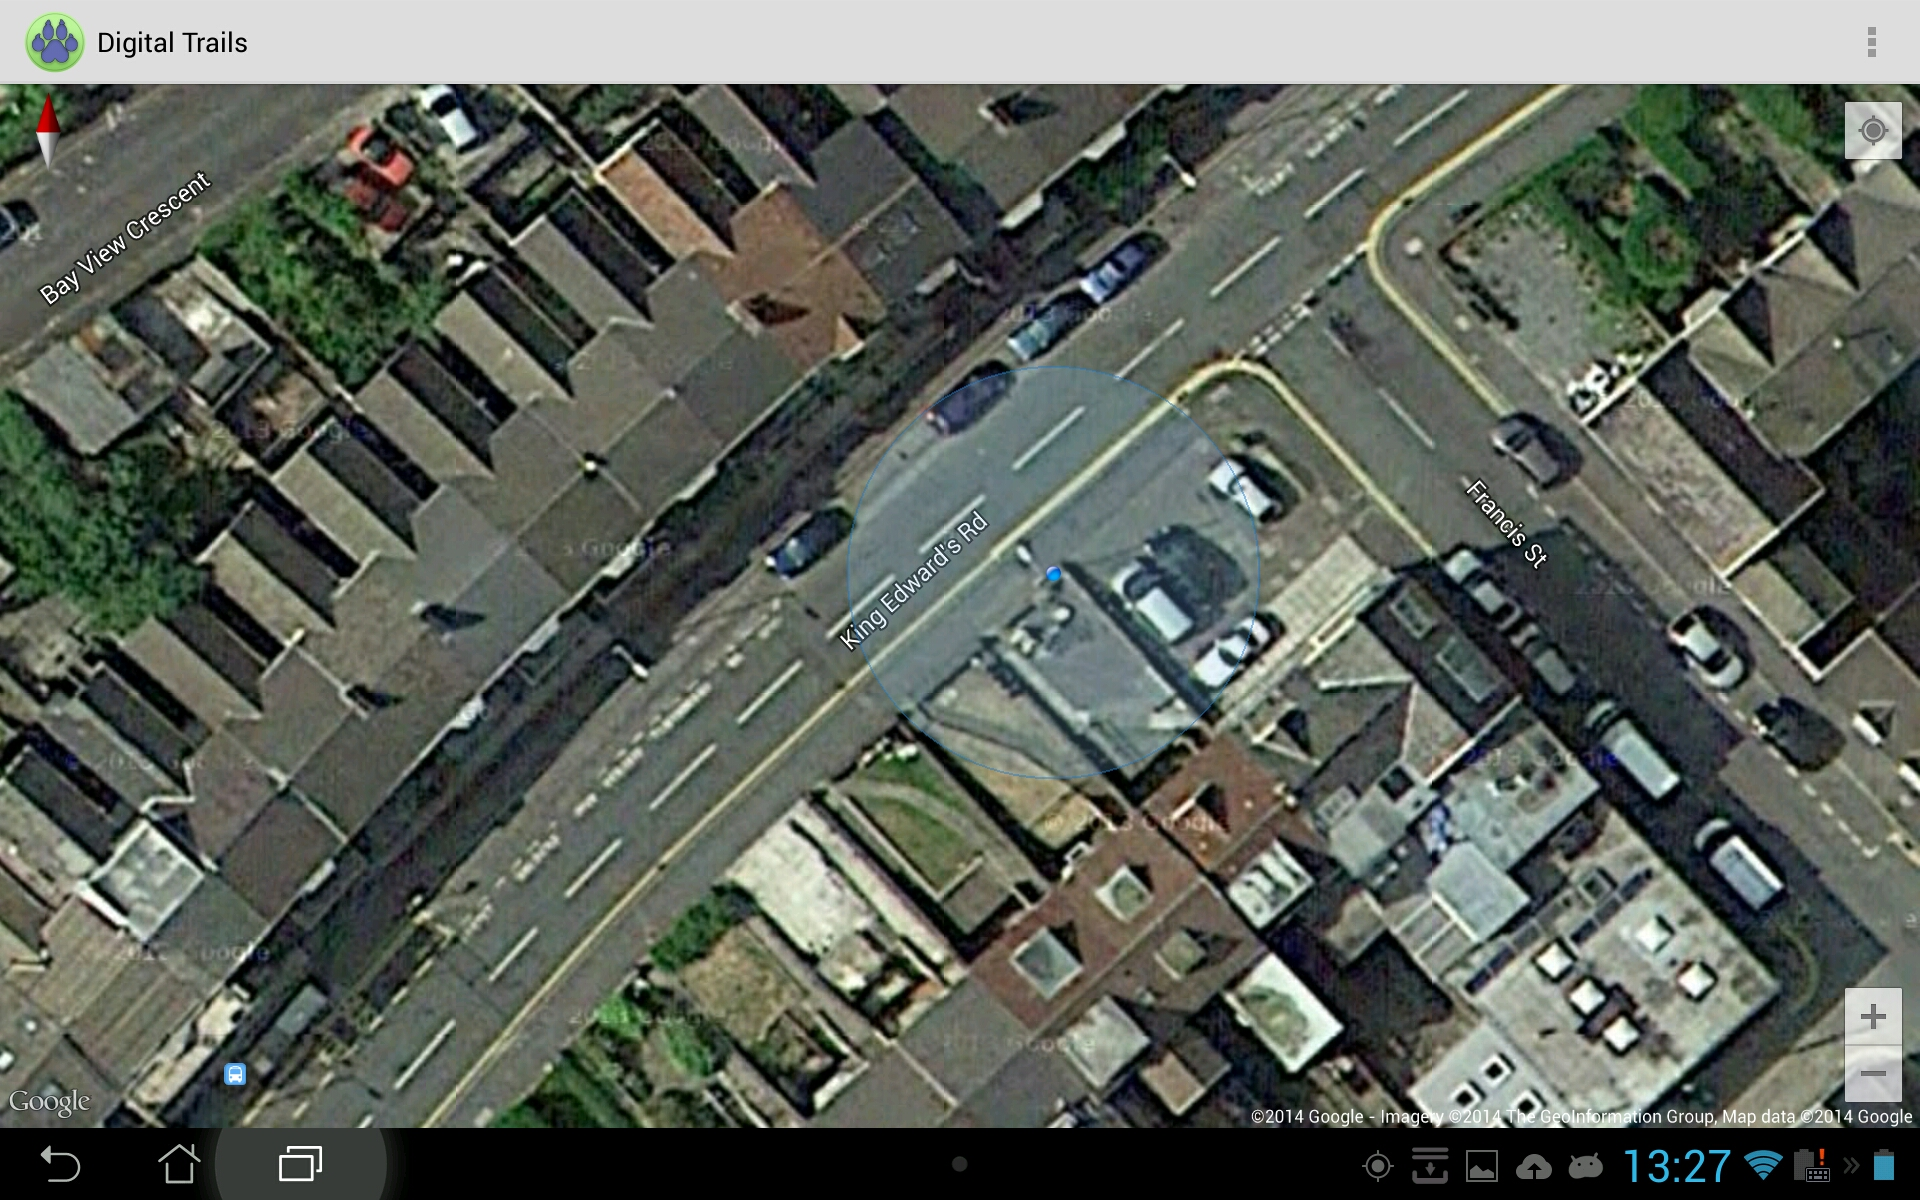
\includegraphics[width=.7\linewidth]{userLocation.jpg}
\caption{Screenshot of the MapActivity displaying user's current location.}
\label{fig:userLocation}
\end{figure}

Future development includes creating a custom InfoWindowAdapter for the InfoWindow, allowing for more customisable data to be displayed. The next waypoint to visit shall be displayed in a different colour than the other waypoints, whilst previously visited waypoints will also change colour.

\subsection{Authentication}
\label{sec:authorisation}
The application needs to interface with the API using the correct authentication method. To achieve this a secureHTTP utility class was created. This classes provides a static method which will take the logged in users account as an object and the http request that needs to be sent. It will then process the request to generate the signature of the data and append the correct headers. The request can then be sent as normal. This utility class also provides the methods for generating the users Private key based upon the password they have entered and for calling the session method on the API to ensure the password is correct without calling any methods which may alter data. 

This class uses several cryptography libraries to ensure that it correctly mimics the action of the web portal and works with the API. The methods are provided as static so they can be used throughout the project wherever a secure API method is needed.

\subsection{SyncAdapter}
\label{sec:syncAdapter}
Whilst the SyncAdaper is not currently implemented, the ContentProvider and Authentication systems are a vital part of this system and it is the foremost reason the ContentProvider was created. The SyncAdapter handles background synchronisation of data from the Android application to the tablet and vice-versa. It is triggered when needed, scheduled or requested. It is the preferred system compared to using Services and IntentServices as it provides an implementation which is:
\begin{itemize}
\item \textbf{Battery Efficient} By being scheduled to run when other synchronisations run, the application is conserving battery power by leaving the device sleeping for as long as possible.
\item \textbf{User Friendly} The SyncAdapter may be accessed by the user from the Android Settings screen, allowing for customisation of the SyncAdapter's settings and even the ability to disable it.
\item \textbf{Content Aware} The ContentProvider which has been written will allow the SyncAdapter to monitor the data and only synchronise with the remote server when the data has been updated.
\item \textbf{Capable of Retrying} The implementation of a SyncAdapter provides it with a retry mechanism, allowing for data to be synchronised as soon as possible.
\end{itemize}

Further information can be found at \url{http://developer.android.com/training/sync-adapters/index.html}.

\subsection{Fragments}
\label{sec:fragments}
Fragments were introduced to several interface views. A fragment can be thought of as a section or portion of an interface view of an activity. Multiple fragments can be used for any given activity. These fragments can then be used across multiple activities, making them efficient and more suitable to use over standard custom views. Having its own life-cycle, a fragment receives its own input events, making it a form of ``sub-activity''. The main advantage of using fragments is that it allows for applications to be written that can scale across multiple screen sizes. Below is a snippet of fragment code used to create the search interface view. It contains two fragments, each with its own layout held in separate XML file.

\lstset{language=xml,
keywordstyle=\color{Maroon},
commentstyle=\color{OliveGreen},
showstringspaces=false, tabsize=4, breaklines=true, showspaces=false, stringstyle=\color{Blue}}
\begin{lstlisting}[captionpos=b, caption=Fragment Code Snippet, label=lst:Fragment Code Snippet, frame=single]
<LinearLayout
    android:orientation="horizontal" >

    <fragment
        android:id="@+id/listFragment"
        class="uk.co.tmilner.whiterock.SearchListFragment" >
    </fragment>

    <fragment
        android:id="@+id/detailFragment"
        class="uk.co.tmilner.whiterock.SearchDetailFragment" >
    </fragment>

</LinearLayout>
\end{lstlisting}

\section{Web Portal Progress}
\label{sec:web-portal}

%- What progress has been made on the web portal?
This section discusses the progress which has been towards development of the web portal. The web portal will allow users of the Android application, full control over the management of their walks. This includes the addition and modification of walks, contributions to other user's walks and the attachment of media such as video, images and audio to specific way points. The web portal aims to provide users with a more intuitive interface to manage walks since the modification of data can be difficult through mobile devices with small screens.

%- Currently what does the portal allow users to do?
A number of features have been developed thus far, including login, registration, responsive layouts, form validation and walk views. Figure \ref{fig:home} shows the first web pages that users will be greeted with upon visiting the web portal. As shown in the diagram, the web portal features distinct White Rock Trails branding which has been designed specifically for this project. This is also a requirement of the software as requested by the client. The visual theme and layout of the web portal has been designed to imitate that of the Android application. This will make the web portal more intuitive to users and its learning curve will be significantly reduced.

%- What tools have been used to create it?
An IDE (Integrated Development Environment) called Brackets was used to develop the web portal. This software features automatic code completion for JavaScript and GIT integration. The former greatly enhanced development productivity while the latter allowed for easy code collaboration between the programming team. The web portal is currently hosted on a public Amazon EC2 server. This allows the client to interact with the latest web portal version and suggested improvements or alterations.

\subsection{Welcome View}

The welcome view shown in Figure \ref{fig:home} provides visitors with a link to download the Android application and instructs them to login or register account in order to use the portal. A footer has also been added to provide users with navigation links to important resources such as the Android application and \emph{About} page.

\begin{figure}[H]
\centering
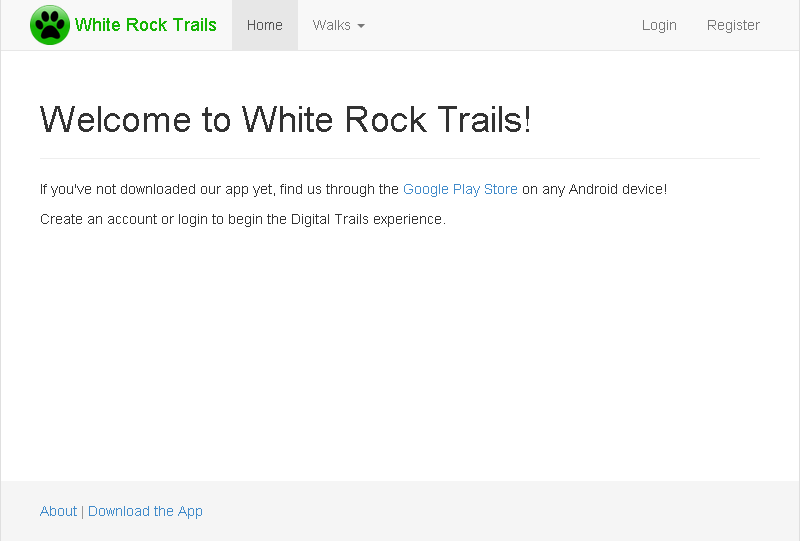
\includegraphics[width=0.8\linewidth]{./img/webportal/home}
\caption{Home view of the web portal.}
\label{fig:home}
\end{figure}

\subsection{Responsive View}

Figure \ref{fig:home-responsive} demonstrates a responsive review of the web portal. This is the view that users will see when visiting the web portal on mobile devices such as smart phones and tablets. The responsive design minimizes the menu bar which can be expanded by clicking the button shown in the top right of the figure. In addition, web page content reduces in width and elements become stacked allowing for easier scrolling on mobile devices. The responsive design of the web portal is facilitated by the Bootstrap (see section \ref{sec:ui-framework}) CSS and JavaScript library.

\begin{figure}[H]
\centering
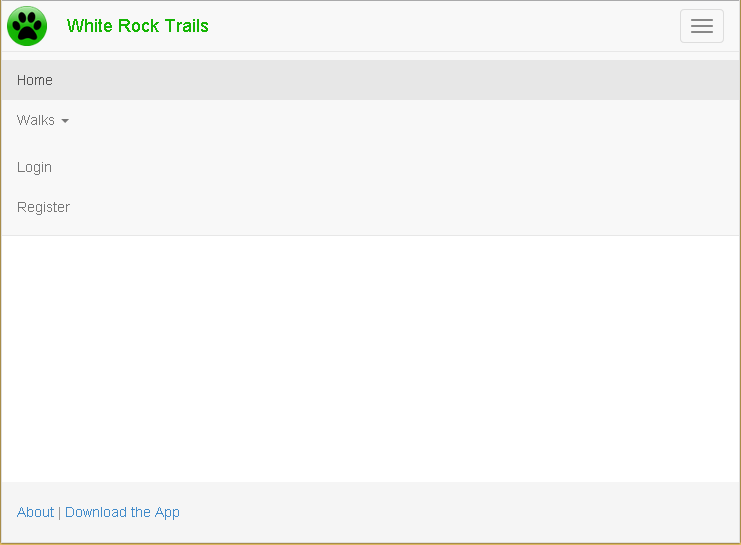
\includegraphics[width=0.8\linewidth]{./img/webportal/home-responsive}
\caption{Web portal responsive menu view.}
\label{fig:home-responsive}
\end{figure}

\subsection{Login View}

Figure \ref{fig:login} shows the login view that users will see when they click on the \emph{Login} button in the top navigation bar. The login view displays as a modal in front of the web page. This will ensure that users do not have to navigate between pages in order to log in, thus enhancing usability. The login view requires users to input their email address and password followed by clicking the \emph{Login} button. The \emph{Login} button will display a spinner icon whilst the fields are validated to ensure the user is aware that the page is loading. An external validation library is used to validate the fields and display an error or success status. The library uses pre-defined validators to validate the structure of the email address and that the email and password pair is valid when checked against the White Rock Trails API. The validator changes the display of erroneous fields to feature red or green borders and tick or cross icons for invalid and valid fields respectively. A specific error message will also be displayed underneath erroneous fields to inform the reason for the error and allow users to amend it. When users successfully log in, the modal will close and the \emph{Login} and \emph{Registration} buttons shown in the top navigation bar are replaced with the user's full name.

\begin{figure}[H]
\centering
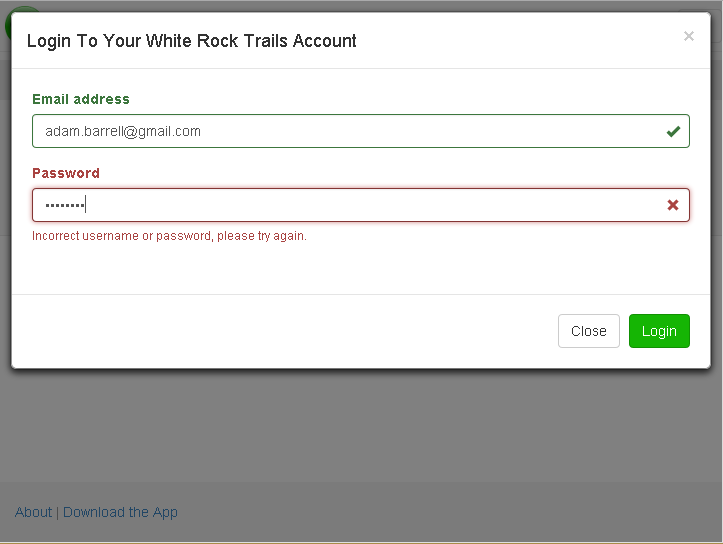
\includegraphics[width=0.8\linewidth]{./img/webportal/login}
\caption{Web portal login modal demonstrating validation.}
\label{fig:login}
\end{figure}

\subsection{Registration View}

Figure \ref{fig:registration} shows the registration view that users will see when the \emph{Register} button is clicked in the top navigation bar. This view is also implemented as a modal for the same reasons as the login view and to maintain consistency throughout the application. The same validator is also used to validate the registration fields. However, inputs such as \emph{Email Address} and the two password fields require different validators. The former uses a validator that checks whether the provided email address has already been registered by another user. The latter checks whether the two passwords are identical. This will prevent users from registering using a mistyped password and subsequently not being able to log in. Clicking the \emph{Register} button will display a loading spinner inside as described for the login view. When users successfully register, they will be presented with a new confirmation modal instructing them to log in with their new account.

\begin{figure}[H]
\centering
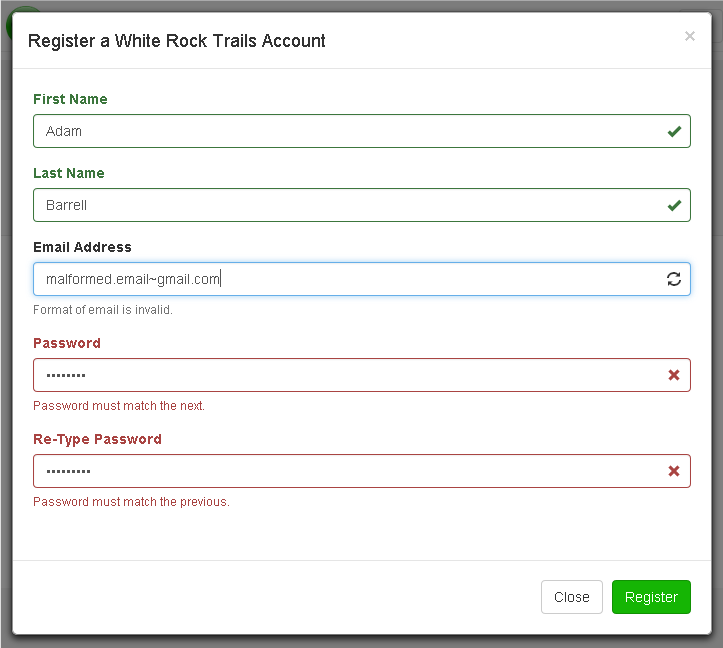
\includegraphics[width=0.8\linewidth]{./img/webportal/registration}
\caption{Web portal registration modal demonstrating validation.}
\label{fig:registration}
\end{figure}

\subsection{All Walks View}

Figure \ref{fig:all-walks} shows the view users will see when they click on the \emph{Walks} button in the top menu bar and select the \emph{All Walks} option. This view displays a list of tiles, each representing a walk in the database. The background of each tile is an image selected from the collection of each walks way point images. Clicking a tile will navigate the user to a walk information view as presented in Figure \ref{fig:walk-info}. The \emph{Add Walk} button and search bar are currently non-functional as those features have not yet been implemented.

\begin{figure}[H]
\centering
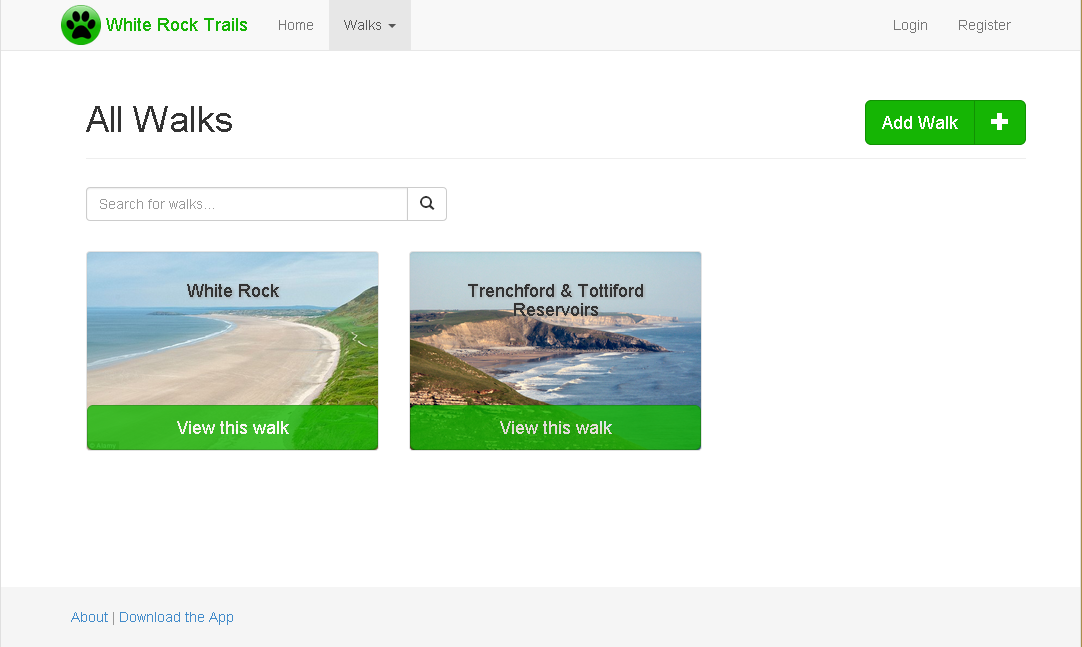
\includegraphics[width=0.8\linewidth]{./img/webportal/all-walks}
\caption{All walks view of the web portal.}
\label{fig:all-walks}
\end{figure}

\subsection{Walk Information View}

Figure \ref{fig:walk-info} shows the view users will see when they click on a walk tile from the \emph{All Walks} view. As shown in the figure, walk information will be displayed in this view such a title, description, duration, distance, difficulty rating and author. Navigation tabs above this information allow users to navigate between the \emph{Waypoints}, \emph{Reviews} and \emph{Walk} views. Walk data is asynchronously loaded from the database through the API. The Google Maps API is used to display the map shown in the right of the figure. The Google Maps API allows markers to be placed at specific GPS locations contained within the walk data. The map allows users to scroll and zoom around the walk area to gain an understanding of its location.

\begin{figure}[H]
\centering
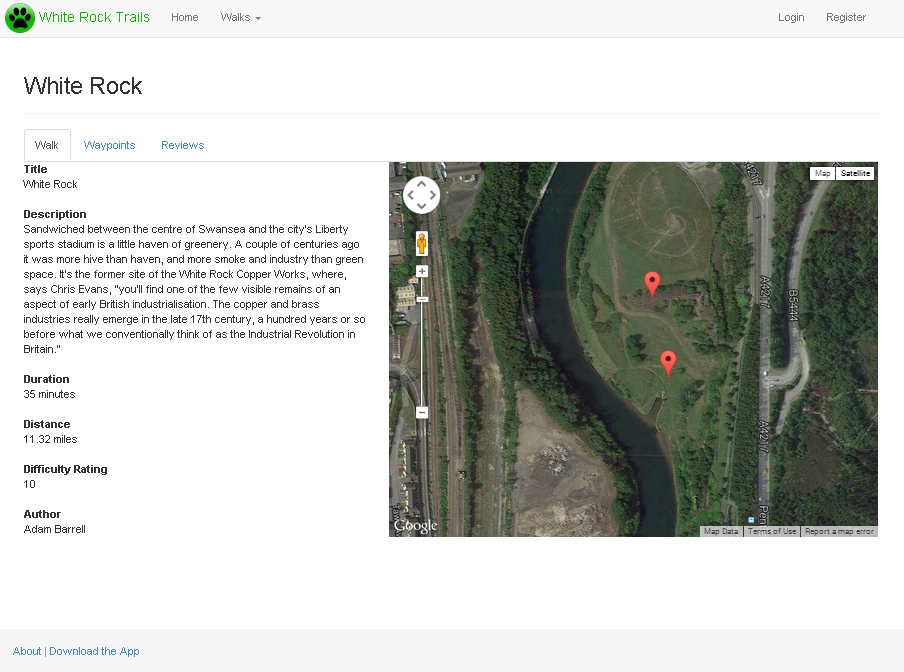
\includegraphics[width=0.8\linewidth]{./img/webportal/walk-info}
\caption{Walk information view of the web portal.}
\label{fig:walk-info}
\end{figure}

\subsection{Walk Way Points View}

Figure \ref{fig:walk-waypoints} shows the view that users will see when they click on the \emph{Waypoints} tab of the walk information view. The view shows the list of way points that are represented by markers on the map. Clicking a list item or its corresponding map marker will display a modal containing media uploaded to the way point such as images, videos and audio. However, this feature is still in progress and is not shown in this document.

\begin{figure}[H]
\centering
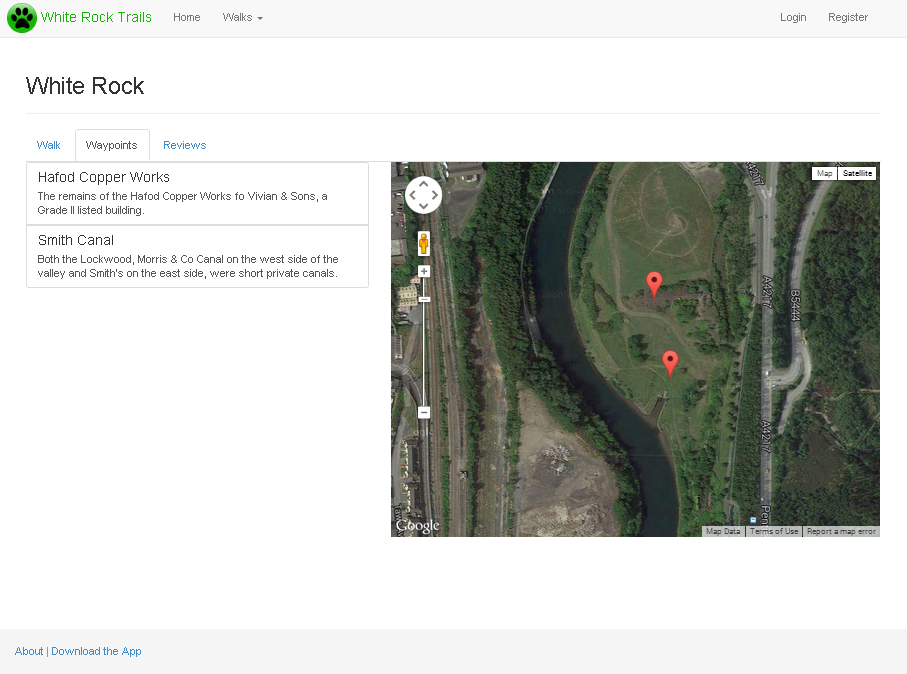
\includegraphics[width=0.8\linewidth]{./img/webportal/walk-waypoints}
\caption{Walk way points view of the web portal.}
\label{fig:walk-waypoints}
\end{figure}

\subsection{Walk Reviews View}

Figure \ref{fig:walk-reviews} shows the view that users will see when they click the \emph{Reviews} tab from the navigation tabs bar. This view loads user reviews from the walk data and displays them in a list view as shown in the figure. A library called \emph{Raty} was used to generate the star rating system seen below the title of the review. It takes a review rating integer between 1-5 and generates a star representation.

\begin{figure}[H]
\centering
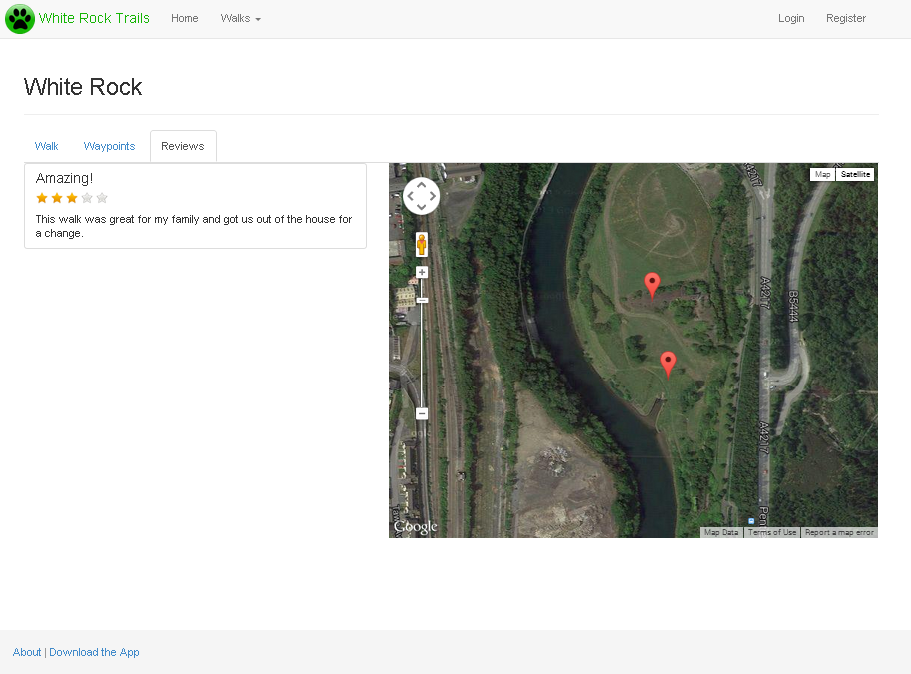
\includegraphics[width=0.8\linewidth]{./img/webportal/walk-reviews}
\caption{Walk reviews view of the web portal.}
\label{fig:walk-reviews}
\end{figure}


\section{Coding Guidelines}
\label{sec:codingguidelines}
A set of coding guidelines have been created for both the Android and Web applications. This will ensure that developers can quickly adapt to and understand the code of team members, reducing unnecessary downtime and interruptions. The main rule of the guidelines is to practice a consistent coding style, which is to say that newly written code should be consistent with the code that is being modified as well as consistent when looked at alone.
\subsection{Android}
\begin{itemize}
\item \textbf{Declaring Variables}
	\begin{enumerate}
	\item All non-static, non-public member variables begin with a lower case m (e.g. mMyVariable).
	\item All static variables begin with a lower case s (e.g. sStaticClass).
	\item All class member variables are private.
	\item Variable names begin with a lower case letter, then each consecutive word in the variable's name begins with an upper-case letter.
	\item Each variable will be declared on a separate line.
	\item A variable should be declared only when needed.
	\item Variable names should be as descriptive as possible, avoid unnecessary abbreviations.
	\item Classes always begin with an upper-case letter.
	\item File names always match class names.
	\item Constant variables are defined in upper-case, with an underscore between words.
	\end{enumerate}
\item \textbf{Whitespace}
	\begin{enumerate}
	\item Always use a single space after a keyword and before a curly brace.
	\end{enumerate}
\item \textbf{Braces}
	\begin{enumerate}
	\item The opening brace goes on the same line as the statement, as is traditional in Java.
	\item Always use curly braces for conditional statements, even if it only contains one line.
	\end{enumerate}
\item \textbf{Documentation}
	\begin{enumerate}
	\item All methods and variables are to be documented with Doxygen, using standard Javadoc style comments.
	\end{enumerate}
\end{itemize}

\subsection{HTML}
\begin{itemize}
\item \textbf{General}
	\begin{enumerate}
	\item Always use lower case for tags.
    \item Always use HTML5
    \item Provide alternative content for all multimedia.
    \item All styling should be done through CSS.
	\end{enumerate}
\item \textbf{Whitespace}
	\begin{enumerate}
    \item Always use a single tab for each level of indentation.
    \item Nested tag blocks should be indented on different lines.
    \item Layout blocks should be separated by a single line.
	\end{enumerate}
\item \textbf{Documentation}
	\begin{enumerate}
	\item Code should be briefly documented to make the structure obvious.
	\end{enumerate}
\end{itemize}

\subsection{CSS}
\begin{itemize}
\item \textbf{General}
	\begin{enumerate}
	\item Always use valid CSS where possible.
    \item Always use meaningful class and ID names.
    \item Avoid type selectors before class and ID names.
    \item Do not specify a unit after a 0 value.
    \item Use short hand properties where possible.
    \item Separate words in ID and class names by a hyphen.
    \item Group sections of rules with section comments.
	\end{enumerate}
\item \textbf{Whitespace}
	\begin{enumerate}
    \item Always use a single tab to indent block contents.
    \item Rules should be separated by a single line.
    \item Selectors should be on a different line to declarations.
	\end{enumerate}
\item \textbf{Documentation}
	\begin{enumerate}
	\item Code should be briefly documented to make the structure obvious.
    \item Any hacks or tricks should be documented fully.
	\end{enumerate}
\end{itemize}

\subsection{JavaScript}
\begin{itemize}
\item \textbf{Declaring Variables}
	\begin{enumerate}
	\item Always use var when defining a variable.
    \item Variable names begin with a lower case letter, then each consecutive word in the variable's name begins with an upper-case letter (CamelCase).
    \item A variable should be declared only when needed.
   	\item Variable names should be as descriptive as possible, avoid unnecessary abbreviations.
	\end{enumerate}
\item \textbf{Whitespace}
	\begin{enumerate}
	\item Always use a single space after a keyword and before a curly brace.
    \item Always use a single tab for each level of indentation.
    \item A space should always be used between function parameters.
    \item A maximum of 2 lines between functions and other code blocks.
	\end{enumerate}
\item \textbf{Braces}
	\begin{enumerate}
	\item The opening brace goes on the same line as the statement.
	\item Always use curly braces for conditional statements, even if it only contains one line.
	\end{enumerate}
\item \textbf{Documentation}
	\begin{enumerate}
	\item All methods and variables are to be documented with Doxygen.
	\end{enumerate}
\end{itemize}

\subsection{PHP}
%Tom
\begin{itemize}
\item \textbf{Declaring Variables}
	\begin{enumerate}
	\item All non-static, non-public member variables begin with a lower case m (e.g. mMyVariable).
	\item All static variables begin with a lower case s (e.g. sStaticClass).
    \item All constants are defined in upper-case, with an underscore between words (e.g. CONSTANT\_VAR).
	\item Variable names begin with a lower case letter, then each consecutive word in the variable's name begins with an upper-case letter (CamelCase).
	\item Each variable will be declared on a separate line.
	\item A variable should be declared only when needed.
	\item Variable names should be as descriptive as possible, avoid unnecessary abbreviations.
	\item Classes always begin with an upper-case letter.
	\item File names always match class names.
	\end{enumerate}
\item \textbf{Whitespace}
	\begin{enumerate}
	\item Always use a single space after a keyword and before a curly brace.
    \item Always use a single tab for each level of indentation.
    \item A space should always be used between function parameters.
    \item A maximum of 2 lines between functions and other code blocks.
	\end{enumerate}
\item \textbf{Braces}
	\begin{enumerate}
	\item The opening brace goes on the same line as the statement.
	\item Always use curly braces for conditional statements, even if it only contains one line.
	\end{enumerate}
\item \textbf{Documentation}
	\begin{enumerate}
	\item All methods and variables are to be documented with Doxygen.
	\end{enumerate}
\end{itemize}


\section{Risk Analysis Review}
\label{sec:risks}
The project has encountered a selection of the risks outlined in the initial document. These risks are:
\begin{itemize}
\item\textbf{TECRSK1} Tesco Hudl fails. The Hudl has began to experience a fault which causes part of the screen to become unresponsive to user input.
\item\textbf{TECRSK2} Personal computers used for software development fail. This has occurred to Adam Barrell on at least one occasion. Thomas Milner has also had his server break, requiring it to be fully reconfigured. This cost us a day of development on the authentication system.
\item\textbf{TECRSK7} The Google Android API is too limited. This is true of the Google Maps API, it does not let the developer extend the Marker class, which would make development easier, nor does it allow for caching of map data for offline use, preventing a serious issue for trails which are in a location that does not receive a mobile data connection. There is, currently, a potential solution which lets us store cached data for a short period of time.
\end{itemize}
The team has also encountered unforeseen risks, detailed below:
\begin{itemize}
\item\textbf{Hudl Support} The Hudl is not seen as a developer device by Tesco, as a result they do not provide a USB driver. A workaround was discovered by forcing the development machine to install the generic Google USB driver to the device.
\item\textbf{Work Environment} The Swansea University Project Lab has been in a contentious state since the beginning of this academic year, with some staff claiming it is a common room whilst other claim it is for group project work. This left developers without a peaceful place to work, as a group, whilst on campus. This has, hopefully, since been rectified after the status of the room was confirmed with members of staff as a room to be used as a working environment.
\item\textbf{Bugs in Libraries} The validation library being used for the website (Bootstrap Validator\cite{bootstrapValidator}) contained a number of bugs, delaying development of the website by a number of days whilst a bug report was processed by the library developer.
\item\textbf{AJAX Cross Origin Resource Sharing} CORS is part of the security infustructure on the web. It caused several issues where it blocked communication with the API. This has since been fixed as the correct headers have been setup. 
\item\textbf{Git User Error} Whilst not a risk which has yet caused a fatal incident, there have been times where user error has caused a delay whilst the local and remote Git repositories are restored to a working state.
\item\textbf{Lab Computers Have Restrictive Permissions} As the lab computers are so restrictive, the development team has not been able to implement the previously mentioned workaround for the Hudl device on one of the Swansea University computers. This prevents developers from using these systems for development. It is also not possible to install new software as required, which includes libraries, thus further increasing the difficulty in which these machines can be used.
\item\textbf{Communication Between Server and Android} This feature has shown itself to require more time than initially expected, to be efficient in both battery and data usage a ContentProvider and SyncAdapter have to be implemented. This adds extra layers of abstraction between the database and the application.
\item\textbf{Initial Code} The initial code the team was given to build upon was not sufficient to continue development, all the data had been hard-coded and strongly died to the OpenStreetMaps implementation. After analysing, commenting and reviewing the code it was deemed faster to begin with a new codebase, capable of using a ContentProvider and SyncAdapter to handle data.
\end{itemize}

\section{Project Schedule Review}
\label{sec:schedule}
%Introduce section
This section will review the project schedule outlined in the initial document of this project. Currently, it is too difficult to assess precisely whether the project is on schedule. The user interfaces and business logic of the Android application are being developed in parallel by two different developers. At the time of writing, the merging process of these two subsystems has only recently begun. Therefore, a time frame is too difficult to predict as the complexity of this process is not yet known. In addition, the complexity of a synchronisation solution for the database and Android application is yet to be completed and forms a major milestone in the development process. Progress on the web portal however, is on schedule and is discussed in section \ref{sec:web-portal}.

%- Client feedback so far, previous client meetings, planned meetings, launch event we attended etc.
The client met in person with the development team on the 26th of February and reviewed the progress that had been achieved. The client was satisfied with the amount of progress made on both the Android application and web portal.  He also brought three target devices (Tesco Hudl) to install the application on for demonstration to the White Rock Trails committee.

The development team attended a White Rock Digital Trails Celebration Event which was held on Saturday 1st of February 2014 at the Swansea Museum Collection Centre in Landore. The event featured some short talks and speeches from the White Rock team followed by a buffet lunch. The development team was present at this event to demonstrate the Android application and web portal to guests of the event. A Tesco Hudl and smart phone was used to demonstrate that the application could be run on a variety of different Android devices. All four team members discussed the software with guests and highlighted their responsibilities within the project.

A future meeting will be planned with the client so more complete versions of the Android application and web portal can be demonstrated. This will allow more accurate feedback to be generated as the client will be able to interact with fully functional prototypes. The feedback from this meeting will be used to revise and enhance the prototype to ensure the software meets the client's requirements and expectations.

%- What user storys have been completed
Figure \ref{fig:UserStoryProgress} demonstrates the progress made developing the user stories of the White Rock Digital Trails software. The figure is a screen capture of the Scrum software that the team is using to manage the delegation and tracking of development tasks. The leftmost column contains user stories that have not yet been developed. The centre column shows those that are currently in progress and being developed. Finally, the rightmost column contains user stories that are fully complete and tested.

\begin{figure}[H]
\centering
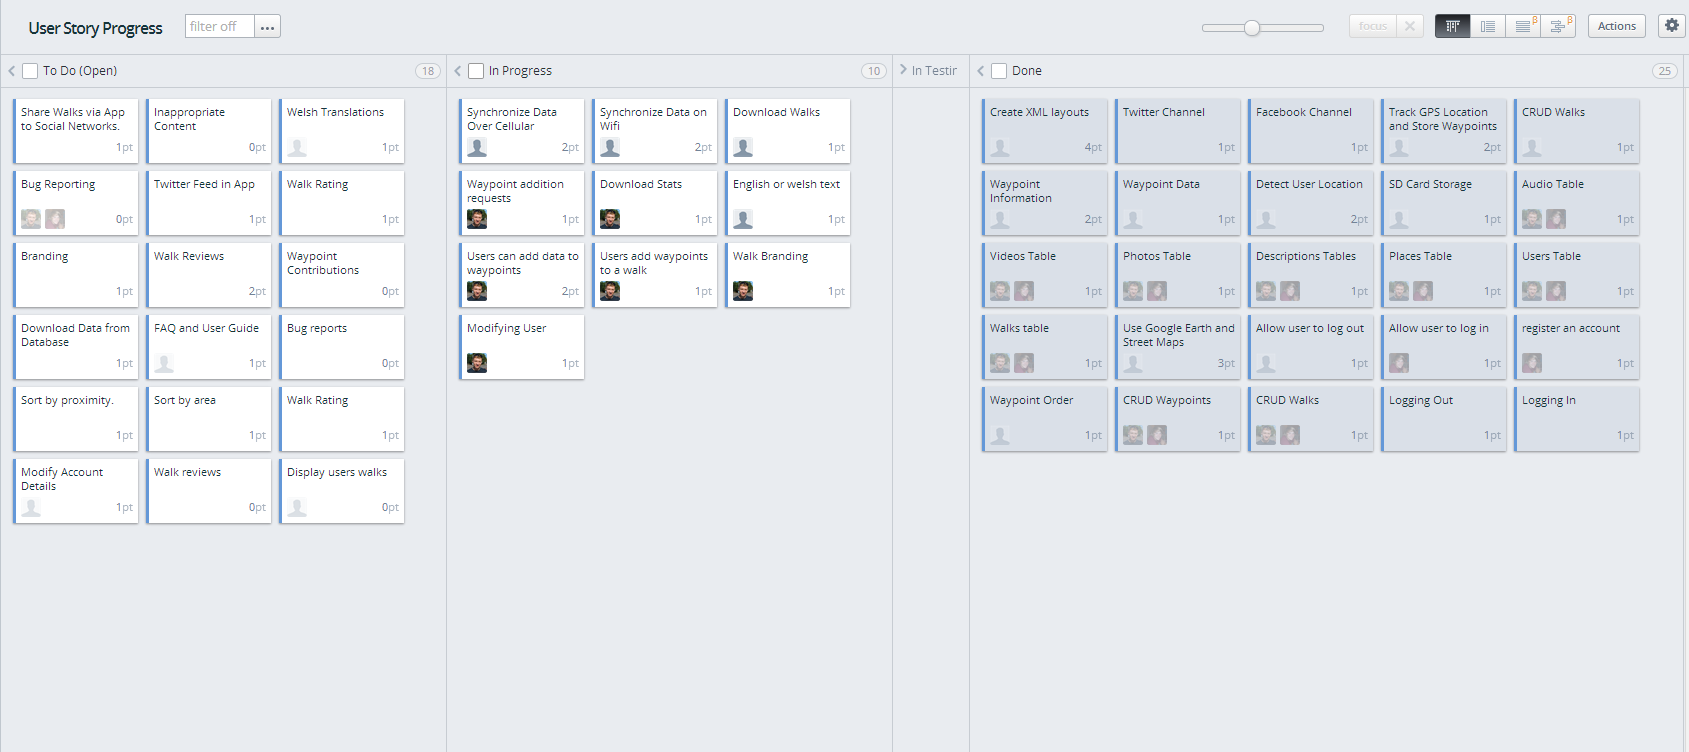
\includegraphics[width=0.9\linewidth]{./img/UserStoryProgress}
\caption{Software development user story progress.}
\label{fig:UserStoryProgress}
\end{figure}


\subsubsection{Software Development Timetable}
\label{sec:plan-software-dev}

This section presents a revised timetable that will be used for the development of the Digital Trails software. This timetable remains for the majority, the same as that outlined in the initial document of this project with the addition of more client meetings and a demonstration event. Tasks are time boxed and given a start and end date for which they must be completed in for the project to deliver on time. As the development team are using 1-2 week sprints based on the amount of work that needs to be done, an abstract time box is defined for each sprint activity. Sprints will run from the start date until the end date by which time the final software should be delivered \cite{initialDoc}.

The revised timetable presented in Figure \ref{fig:software-dev-table} reflects the addition of two tasks, namely the \emph{White Rock Demonstration} and \emph{Client Meeting 4}. The former required the development team to demonstrate progress made on the Android application and web portal to members of the White Rock team at a celebration event. The latter involved a brief meeting to demonstrate further progress to the client where the team received feedback on the current state of the software.

\renewcommand{\arraystretch}{1.5}
\newcommand*{\tableIndent}{\hspace*{0.4cm}}

\begin{figure}[H]
\centering
\begin{tabular}{|l|l|l|}
\hline \textbf{Task} & \textbf{Start Date} & \textbf{End Date} \\
\hline\hline{Client Meeting 1} & \multicolumn{2}{c|}{25 Oct 2013} \\
\hline{Client Meeting 2} & \multicolumn{2}{c|}{15 Nov 2013} \\
\hline{Client Meeting 3} & \multicolumn{2}{c|}{14 Jan 2014} \\
\hline{White Rock Demonstration} & \multicolumn{2}{c|}{1 Feb 2014} \\
\hline{Client Meeting 4} & \multicolumn{2}{c|}{25 Feb 2014} \\
\hline \multirow{2}{*}{\textbf{Sprints}} & \multicolumn{2}{c|}{1-2 Week Iterations} \\ \cline{2-3}
 & 22 Jan 2014 & 09 May 2014 \\
\hline\tableIndent{Backlog Refinement} & \multicolumn{2}{c|}{4 Hours} \\
\hline\tableIndent{Analyse} & \multicolumn{2}{c|}{4 Hours - 1 Day} \\
\hline\tableIndent{Develop} & \multicolumn{2}{c|}{3-9 Days} \\
\hline\tableIndent{Test} & \multicolumn{2}{c|}{1-2 Days} \\
\hline\tableIndent{Client Feedback} & \multicolumn{2}{c|}{4 Hours - 1 Day} \\
\hline\tableIndent{Deploy} & \multicolumn{2}{c|}{2-4 Hours} \\
\hline
\end{tabular}
\caption{Software development time table.\label{fig:software-dev-table}}
\end{figure}

\subsection{Requirements Progress}

This section outlines the progress made towards completion of each requirement defined in the initial document\cite{initialDoc}. All requirements have remained the same as those defined in the initial document as the client has not requested any changes during development.

%- What reqs are completed Chris Lewis' favourite job!).
\subsubsection{Web Portal}

\begin{longtable}{ p{0.14\textwidth}|p{0.2\textwidth}|p{0.58\textwidth} }
\textbf{Code} & \textbf{Status} & \textbf{Comment} \\
\hline
WEBREQ1 & Complete & The web portal allows users to register a new account. \\ \hline
WEBREQ2 & Complete & The web portal allows registered users to log in. \\ \hline
WEBREQ3 & Complete & The web portal allows registered users to log out. \\ \hline
WEBREQ4 & Not Implemented & The web portal does not allow registered users to modify their account details. \\ \hline
WEBREQ5 & Complete & The web portal interface features distinctive White Rock branding. \\ \hline
WEBREQ6 & Not Implemented & The web portal does not allow registered users to add sub-branding to created walks. \\ \hline
WEBREQ7 & In Progress & The web portal navigation bar contains a link to the users walk contributions page, however the page has not been created yet. \\ \hline
WEBREQ8 & Not Implemented & The web portal does not allow registered users to create, edit and delete their own walks. \\ \hline
WEBREQ9 & Not Implemented & The web portal does not allow registered users to create, edit and delete their own waypoints. \\ \hline
WEBREQ10 & Not Implemented & The web portal does not allow registered users to add GPS waypoints to a walk. \\ \hline
WEBREQ11 & Not Implemented & The web portal does not allow registered users to modify the order each waypoint should be visited. \\ \hline
WEBREQ12 & Not Implemented & The web portal does not allow registered users to upload, edit and delete waypoint data such as images, text, audio and video. \\ \hline
WEBREQ13 & Not Implemented & The web portal should allow registered users to provide English and Welsh translation for text. \\ \hline
WEBREQ14 & Completed & The web portal displays download statistics for each of the user's walks. \\ \hline
WEBREQ15 & Completed & The web portal displays reviews for each of the user's walks. \\ \hline
WEBREQ16 & Not Implemented & The web portal does not display an average rating for each of the user's walks. \\ \hline
WEBREQ17 & Not Implemented & The web portal does not notify registered users of waypoint addition requests. \\ \hline
WEBREQ18 & Not Implemented & The web portal does not allow registered users to accept or reject requested waypoint additions. \\ \hline
WEBREQ19 & Not Implemented & The web portal does not allow registered users to report bugs and errors. \\ \hline
WEBREQ20 & Not Implemented & The web portal does not contain a FAQ and user guide. \\
\end{longtable}

\subsubsection{Android Application}
\label{sec:app-reqs}

\begin{longtable}{ p{0.14\textwidth}|p{0.2\textwidth}|p{0.58\textwidth} }
\textbf{Code} & \textbf{Status} & \textbf{Comment} \\
\hline
APPREQ1 & Completed & The application allows users to register user accounts. \\ \hline
APPREQ2 & Completed & The application allows registered users to log in. \\ \hline
APPREQ3 & Completed & The application allows registered users to log out. \\ \hline
APPREQ4 & Not Implemented & The application should allow registered users to modify their account details. \\ \hline
APPREQ5 & In Progress & Non functional views have been developed that will allow users to download walks created by registered users. \\ \hline
APPREQ6 & Not Implemented & The application does not group walks by local area. \\ \hline
APPREQ7 & Not Implemented & The application does not sort grouped walks by current proximity to the user. \\ \hline
APPREQ8 & Completed & The application allows users to use Google earth and street maps interchangeably while viewing a walk. \\ \hline
APPREQ9 & Not Implemented & The application does not allow registered users to choose a default map view for a created walk. \\ \hline
APPREQ10 & Not Implemented & The application does not download data from a remote database. \\ \hline
APPREQ11 & Not Implemented & The application does not synchronise data whilst the host device is connected to WiFi. \\ \hline
APPREQ12 & Not Implemented & The application does not give users the option to synchronise data over cellular networks. \\ \hline
APPREQ13 & Not Implemented & The application does not give users the option to store data on a SD card if available. \\ \hline
APPREQ14 & Completed &  The application detects a user's GPS location consistently between devices. \\ \hline
APPREQ15 & Not Implemented & The application does not display the preferred order to visit waypoints in a walk. \\ \hline
APPREQ16 & Not Implemented & The application does not automatically display waypoint information when a waypoint is re-visited. \\ \hline
APPREQ17 & Not Implemented & The application does not allow registered users to create, edit and delete their own walks. \\ \hline
APPREQ18 & Not Implemented & The application does not allow registered users to tag GPS waypoints in their own walks. \\ \hline
APPREQ19 & Not Implemented & The application does not track the order that GPS waypoints were tagged in a created walk. \\ \hline
APPREQ20 & Not Implemented & The application does not allow registered users to upload audio, images and video to a waypoint. \\ \hline
APPREQ21 & Completed & The application does separate audio, images, text and video waypoint data. \\ \hline
APPREQ22 & Completed & The application interface features distinctive White Rock branding. \\ \hline
APPREQ23 & Not Implemented & The application does not allow registered users to contribute waypoints to other user's walks by request. \\ \hline
APPREQ24 & Not Implemented & The application does not allow users to leave reviews of walks. \\ \hline
APPREQ25 & Not Implemented & The application does not allow users to rate walks they have completed. \\ \hline
APPREQ26 & Not Implemented & The application does not allow users to report bugs and errors. \\ \hline
APPREQ27 & Not Implemented & The application does not provide links to the application's Twitter and Facebook channels. \\ \hline
APPREQ28 & In Progress & English and Welsh translations for text is currently in progress. \\ \hline
APPREQ29 & Not Implemented & The application does not allow users to report inappropriate content to an administrator. \\ \hline
\end{longtable}

\subsubsection{Database}
\label{sec:db-reqs}

\begin{longtable}{ p{0.14\textwidth}|p{0.2\textwidth}|p{0.58\textwidth} }
\textbf{Code} & \textbf{Requirement} \\
\hline
DBREQ1 & Completed & The database has the ability to store a walk.\\ \hline
DBREQ2 & Completed & Each walk links to a description.  \\ \hline
DBREQ3 & Completed & The walks table has `Difficultly', `Duration' and `Distance'. \\ \hline
DBREQ4 & Completed & The database has the ability to store a place, which is a location on a walk.\\ \hline
DBREQ5 & Completed & The places table links to a walk.\\ \hline
DBREQ6 & Completed & The places table contains a `Latitude' and `Longitude' to store the position. \\ \hline
DBREQ7 & Completed & The places table links to a description. \\ \hline
DBREQ8 & Completed & The database has the ability to store a description for each supported language. \\ \hline
DBREQ9 & Completed & The descriptions are replicas of each other, but in the correct language. \\ \hline
DBREQ10 & Completed & The descriptions include a `Title', a `Short Description' and a `Description'.\\ \hline
DBREQ11 & Completed & The database has the ability to store photos. \\ \hline
DBREQ12 & Completed & The database has the ability to link photos to places and walks.\\ \hline
DBREQ13 & Completed & The photos store the location of the photo file in the file system.\\ \hline
DBREQ14 & Completed & The database has the ability to store videos. \\ \hline
DBREQ15 & Completed & The database has the ability to link videos to places and walks.\\ \hline
DBREQ16 & Completed & The videos store the location of the video file in the file system.\\ \hline
DBREQ17 & Completed & The database has the ability to store audio. \\ \hline
DBREQ18 & Completed & The database has the ability to link audio to places and walks.\\ \hline
DBREQ19 & Completed & The audio stores the location of the audio file in the file system.\\ \hline
DBREQ20 & Completed & The database has the ability to store Users. \\ \hline
DBREQ21 & Completed & The users have a `Username', an `Email' and a `Password'.\\ \hline
DBREQ22 & Completed & The users link to Walks, Places, Photos, Videos and Audio they add. \\ \hline
DBREQ23 & Completed & The users store related settings. \\ \hline

\end{longtable}

\subsubsection{Non-Functional}
\label{sec:non-func-reqs}

\begin{longtable}{ p{0.14\textwidth}|p{0.2\textwidth}|p{0.58\textwidth} }
\textbf{Code} & \textbf{Status} & \textbf{Comment} \\

\hline
NFREQ1 & In Progress & An agreement with the other development team and client is being discussed with regards to database sharing. \\ \hline
NFREQ2 & Completed & The user interfaces have been designed to be intuitive to users with little technology experience. \\ \hline
NFREQ3 & In Progress & The application is being designed to be usable for visually impaired (colour blind) users. \\ \hline
NFREQ4 & In Progress & The application code is being written to be maintainable for future developers. \\ \hline
NFREQ5 & In Progress & The application code is being fully documented as it is written. \\ \hline
NFREQ6 & Completed & The application currently runs efficiently on lower end GPS-enabled android tablets. \\ \hline
NFREQ7 & Completed & The application currently runs efficiently on android smartphones. \\ \hline
NFREQ8 & Completed & The application is compatible with typical tablet screen sizes. \\ \hline
NFREQ9 & Completed & The application scales well when using typical smart phone screen sizes. \\ \hline
NFREQ10 & In Progress & The application is being developed to be battery efficient by sampling GPS locations based on the user's mode of transport. \\ \hline
NFREQ11 & In Progress & The application is being developed to be bandwidth efficient. \\ \hline
\end{longtable}

%TODO: What sprints we have completed?
\subsection{Sprint Progress}
The majority of sprints have been completed within schedule as defined in the timetable presented in Figure \ref{fig:software-dev-table}. Some sprints however, took longer than anticipated and exceeded the time box they were assigned. For example, the sprint containing the web portal login and registration features was delayed due to technical issues with a third party validation library. More specifically, the library contained bugs which were overlooked by the developer and slowed down the development of these features as a bug fix was required. The time lost during this sprint was recovered in the next sprint as more resources were invested into developing the required features.

\section{Summary}
\label{sec:summary}
As can be seen throughout this document, the project is progressing to a high standard on all fronts. Whilst initial work on the Android application looks to have been slow, in terms of requirements met, the more flexible and higher quality backend of the application will allow for the remaining requirements to be completed at a faster pace than before. This increase in productivity during the latter stages of the project will make up the time spent dealing with the risks detailed in section~\ref{sec:risks}

The development of the web portal has also seen hard times during the first half of development, but like the Android application development can now become more efficient with a solid backend to build upon.

The final release date is May 9th 2014, which the development team still feels is achievable without sacrificing features on either the web portal or Android application.

%References as subsection
\newpage
\bibliographystyle{plain}
\bibliography{bibliography}
\end{document}
